% Created by tikzDevice version 0.6.2-92-0ad2792 on 2013-03-06 14:04:27
% !TEX encoding = UTF-8 Unicode
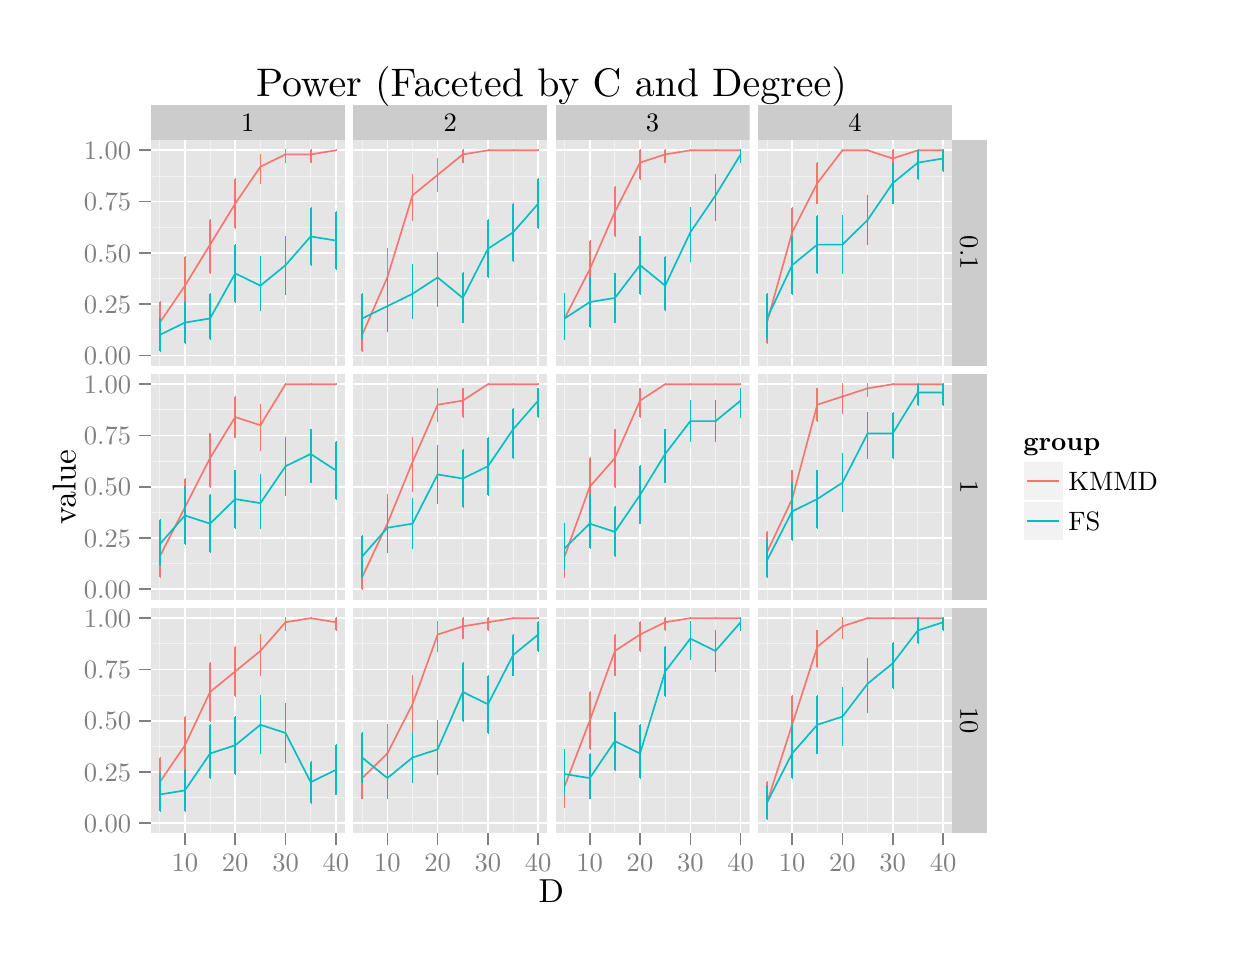
\begin{tikzpicture}[x=1pt,y=1pt]
\definecolor[named]{fillColor}{rgb}{1.00,1.00,1.00}
\path[use as bounding box,fill=fillColor,fill opacity=0.00] (0,0) rectangle (433.62,325.21);
\begin{scope}
\path[clip] (  0.00,  0.00) rectangle (433.62,325.21);
\definecolor[named]{drawColor}{rgb}{1.00,1.00,1.00}
\definecolor[named]{fillColor}{rgb}{1.00,1.00,1.00}

\path[draw=drawColor,line width= 0.6pt,line join=round,line cap=round,fill=fillColor] (  0.00,  0.00) rectangle (433.62,325.21);
\end{scope}
\begin{scope}
\path[clip] ( 44.49,284.60) rectangle (114.61,297.23);
\definecolor[named]{fillColor}{rgb}{0.80,0.80,0.80}

\path[fill=fillColor] ( 44.49,284.60) rectangle (114.61,297.23);
\definecolor[named]{drawColor}{rgb}{0.00,0.00,0.00}

\node[text=drawColor,anchor=base,inner sep=0pt, outer sep=0pt, scale=  0.96] at ( 79.55,287.61) {1};
\end{scope}
\begin{scope}
\path[clip] (117.62,284.60) rectangle (187.75,297.23);
\definecolor[named]{fillColor}{rgb}{0.80,0.80,0.80}

\path[fill=fillColor] (117.62,284.60) rectangle (187.75,297.23);
\definecolor[named]{drawColor}{rgb}{0.00,0.00,0.00}

\node[text=drawColor,anchor=base,inner sep=0pt, outer sep=0pt, scale=  0.96] at (152.68,287.61) {2};
\end{scope}
\begin{scope}
\path[clip] (190.76,284.60) rectangle (260.88,297.23);
\definecolor[named]{fillColor}{rgb}{0.80,0.80,0.80}

\path[fill=fillColor] (190.76,284.60) rectangle (260.88,297.23);
\definecolor[named]{drawColor}{rgb}{0.00,0.00,0.00}

\node[text=drawColor,anchor=base,inner sep=0pt, outer sep=0pt, scale=  0.96] at (225.82,287.61) {3};
\end{scope}
\begin{scope}
\path[clip] (263.89,284.60) rectangle (334.02,297.23);
\definecolor[named]{fillColor}{rgb}{0.80,0.80,0.80}

\path[fill=fillColor] (263.89,284.60) rectangle (334.02,297.23);
\definecolor[named]{drawColor}{rgb}{0.00,0.00,0.00}

\node[text=drawColor,anchor=base,inner sep=0pt, outer sep=0pt, scale=  0.96] at (298.95,287.61) {4};
\end{scope}
\begin{scope}
\path[clip] ( 44.49,203.08) rectangle (114.61,284.60);
\definecolor[named]{fillColor}{rgb}{0.90,0.90,0.90}

\path[fill=fillColor] ( 44.49,203.08) rectangle (114.61,284.60);
\definecolor[named]{drawColor}{rgb}{0.95,0.95,0.95}

\path[draw=drawColor,line width= 0.3pt,line join=round] ( 44.49,216.05) --
	(114.61,216.05);

\path[draw=drawColor,line width= 0.3pt,line join=round] ( 44.49,234.58) --
	(114.61,234.58);

\path[draw=drawColor,line width= 0.3pt,line join=round] ( 44.49,253.10) --
	(114.61,253.10);

\path[draw=drawColor,line width= 0.3pt,line join=round] ( 44.49,271.63) --
	(114.61,271.63);

\path[draw=drawColor,line width= 0.3pt,line join=round] ( 47.74,203.08) --
	( 47.74,284.60);

\path[draw=drawColor,line width= 0.3pt,line join=round] ( 65.91,203.08) --
	( 65.91,284.60);

\path[draw=drawColor,line width= 0.3pt,line join=round] ( 84.09,203.08) --
	( 84.09,284.60);

\path[draw=drawColor,line width= 0.3pt,line join=round] (102.27,203.08) --
	(102.27,284.60);
\definecolor[named]{drawColor}{rgb}{1.00,1.00,1.00}

\path[draw=drawColor,line width= 0.6pt,line join=round] ( 44.49,206.79) --
	(114.61,206.79);

\path[draw=drawColor,line width= 0.6pt,line join=round] ( 44.49,225.31) --
	(114.61,225.31);

\path[draw=drawColor,line width= 0.6pt,line join=round] ( 44.49,243.84) --
	(114.61,243.84);

\path[draw=drawColor,line width= 0.6pt,line join=round] ( 44.49,262.36) --
	(114.61,262.36);

\path[draw=drawColor,line width= 0.6pt,line join=round] ( 44.49,280.89) --
	(114.61,280.89);

\path[draw=drawColor,line width= 0.6pt,line join=round] ( 56.83,203.08) --
	( 56.83,284.60);

\path[draw=drawColor,line width= 0.6pt,line join=round] ( 75.00,203.08) --
	( 75.00,284.60);

\path[draw=drawColor,line width= 0.6pt,line join=round] ( 93.18,203.08) --
	( 93.18,284.60);

\path[draw=drawColor,line width= 0.6pt,line join=round] (111.36,203.08) --
	(111.36,284.60);
\definecolor[named]{drawColor}{rgb}{0.97,0.46,0.43}

\path[draw=drawColor,line width= 0.6pt,line join=round] ( 47.74,218.64) --
	( 56.83,231.98) --
	( 65.91,246.80) --
	( 75.00,261.62) --
	( 84.09,274.96) --
	( 93.18,279.41) --
	(102.27,279.41) --
	(111.36,280.89);
\definecolor[named]{drawColor}{rgb}{0.00,0.75,0.77}

\path[draw=drawColor,line width= 0.6pt,line join=round] ( 47.74,214.20) --
	( 56.83,218.64) --
	( 65.91,220.13) --
	( 75.00,236.43) --
	( 84.09,231.98) --
	( 93.18,239.39) --
	(102.27,249.77) --
	(111.36,248.29);
\definecolor[named]{drawColor}{rgb}{0.97,0.46,0.43}

\path[draw=drawColor,line width= 0.6pt,line join=round] ( 47.67,226.05) --
	( 47.80,226.05);

\path[draw=drawColor,line width= 0.6pt,line join=round] ( 47.74,226.05) --
	( 47.74,211.23);

\path[draw=drawColor,line width= 0.6pt,line join=round] ( 47.67,211.23) --
	( 47.80,211.23);

\path[draw=drawColor,line width= 0.6pt,line join=round] ( 56.76,242.36) --
	( 56.89,242.36);

\path[draw=drawColor,line width= 0.6pt,line join=round] ( 56.83,242.36) --
	( 56.83,223.09);

\path[draw=drawColor,line width= 0.6pt,line join=round] ( 56.76,223.09) --
	( 56.89,223.09);

\path[draw=drawColor,line width= 0.6pt,line join=round] ( 65.85,255.73) --
	( 65.98,255.73);

\path[draw=drawColor,line width= 0.6pt,line join=round] ( 65.91,255.73) --
	( 65.91,236.43);

\path[draw=drawColor,line width= 0.6pt,line join=round] ( 65.85,236.43) --
	( 65.98,236.43);

\path[draw=drawColor,line width= 0.6pt,line join=round] ( 74.94,270.52) --
	( 75.07,270.52);

\path[draw=drawColor,line width= 0.6pt,line join=round] ( 75.00,270.52) --
	( 75.00,252.73);

\path[draw=drawColor,line width= 0.6pt,line join=round] ( 74.94,252.73) --
	( 75.07,252.73);

\path[draw=drawColor,line width= 0.6pt,line join=round] ( 84.03,279.41) --
	( 84.16,279.41);

\path[draw=drawColor,line width= 0.6pt,line join=round] ( 84.09,279.41) --
	( 84.09,269.03);

\path[draw=drawColor,line width= 0.6pt,line join=round] ( 84.03,269.03) --
	( 84.16,269.03);

\path[draw=drawColor,line width= 0.6pt,line join=round] ( 93.12,280.89) --
	( 93.24,280.89);

\path[draw=drawColor,line width= 0.6pt,line join=round] ( 93.18,280.89) --
	( 93.18,276.44);

\path[draw=drawColor,line width= 0.6pt,line join=round] ( 93.12,276.44) --
	( 93.24,276.44);

\path[draw=drawColor,line width= 0.6pt,line join=round] (102.21,280.89) --
	(102.33,280.89);

\path[draw=drawColor,line width= 0.6pt,line join=round] (102.27,280.89) --
	(102.27,276.44);

\path[draw=drawColor,line width= 0.6pt,line join=round] (102.21,276.44) --
	(102.33,276.44);

\path[draw=drawColor,line width= 0.6pt,line join=round] (111.29,280.89) --
	(111.42,280.89);

\path[draw=drawColor,line width= 0.6pt,line join=round] (111.36,280.89) --
	(111.36,280.89);

\path[draw=drawColor,line width= 0.6pt,line join=round] (111.29,280.89) --
	(111.42,280.89);
\definecolor[named]{drawColor}{rgb}{0.00,0.75,0.77}

\path[draw=drawColor,line width= 0.6pt,line join=round] ( 47.67,220.13) --
	( 47.80,220.13);

\path[draw=drawColor,line width= 0.6pt,line join=round] ( 47.74,220.13) --
	( 47.74,208.27);

\path[draw=drawColor,line width= 0.6pt,line join=round] ( 47.67,208.27) --
	( 47.80,208.27);

\path[draw=drawColor,line width= 0.6pt,line join=round] ( 56.76,226.05) --
	( 56.89,226.05);

\path[draw=drawColor,line width= 0.6pt,line join=round] ( 56.83,226.05) --
	( 56.83,211.23);

\path[draw=drawColor,line width= 0.6pt,line join=round] ( 56.76,211.23) --
	( 56.89,211.23);

\path[draw=drawColor,line width= 0.6pt,line join=round] ( 65.85,229.02) --
	( 65.98,229.02);

\path[draw=drawColor,line width= 0.6pt,line join=round] ( 65.91,229.02) --
	( 65.91,212.72);

\path[draw=drawColor,line width= 0.6pt,line join=round] ( 65.85,212.72) --
	( 65.98,212.72);

\path[draw=drawColor,line width= 0.6pt,line join=round] ( 74.94,246.80) --
	( 75.07,246.80);

\path[draw=drawColor,line width= 0.6pt,line join=round] ( 75.00,246.80) --
	( 75.00,226.05);

\path[draw=drawColor,line width= 0.6pt,line join=round] ( 74.94,226.05) --
	( 75.07,226.05);

\path[draw=drawColor,line width= 0.6pt,line join=round] ( 84.03,242.36) --
	( 84.16,242.36);

\path[draw=drawColor,line width= 0.6pt,line join=round] ( 84.09,242.36) --
	( 84.09,223.09);

\path[draw=drawColor,line width= 0.6pt,line join=round] ( 84.03,223.09) --
	( 84.16,223.09);

\path[draw=drawColor,line width= 0.6pt,line join=round] ( 93.12,249.77) --
	( 93.24,249.77);

\path[draw=drawColor,line width= 0.6pt,line join=round] ( 93.18,249.77) --
	( 93.18,229.02);

\path[draw=drawColor,line width= 0.6pt,line join=round] ( 93.12,229.02) --
	( 93.24,229.02);

\path[draw=drawColor,line width= 0.6pt,line join=round] (102.21,260.14) --
	(102.33,260.14);

\path[draw=drawColor,line width= 0.6pt,line join=round] (102.27,260.14) --
	(102.27,239.39);

\path[draw=drawColor,line width= 0.6pt,line join=round] (102.21,239.39) --
	(102.33,239.39);

\path[draw=drawColor,line width= 0.6pt,line join=round] (111.29,258.66) --
	(111.42,258.66);

\path[draw=drawColor,line width= 0.6pt,line join=round] (111.36,258.66) --
	(111.36,237.91);

\path[draw=drawColor,line width= 0.6pt,line join=round] (111.29,237.91) --
	(111.42,237.91);
\end{scope}
\begin{scope}
\path[clip] ( 44.49,118.56) rectangle (114.61,200.07);
\definecolor[named]{fillColor}{rgb}{0.90,0.90,0.90}

\path[fill=fillColor] ( 44.49,118.56) rectangle (114.61,200.07);
\definecolor[named]{drawColor}{rgb}{0.95,0.95,0.95}

\path[draw=drawColor,line width= 0.3pt,line join=round] ( 44.49,131.53) --
	(114.61,131.53);

\path[draw=drawColor,line width= 0.3pt,line join=round] ( 44.49,150.05) --
	(114.61,150.05);

\path[draw=drawColor,line width= 0.3pt,line join=round] ( 44.49,168.58) --
	(114.61,168.58);

\path[draw=drawColor,line width= 0.3pt,line join=round] ( 44.49,187.10) --
	(114.61,187.10);

\path[draw=drawColor,line width= 0.3pt,line join=round] ( 47.74,118.56) --
	( 47.74,200.07);

\path[draw=drawColor,line width= 0.3pt,line join=round] ( 65.91,118.56) --
	( 65.91,200.07);

\path[draw=drawColor,line width= 0.3pt,line join=round] ( 84.09,118.56) --
	( 84.09,200.07);

\path[draw=drawColor,line width= 0.3pt,line join=round] (102.27,118.56) --
	(102.27,200.07);
\definecolor[named]{drawColor}{rgb}{1.00,1.00,1.00}

\path[draw=drawColor,line width= 0.6pt,line join=round] ( 44.49,122.26) --
	(114.61,122.26);

\path[draw=drawColor,line width= 0.6pt,line join=round] ( 44.49,140.79) --
	(114.61,140.79);

\path[draw=drawColor,line width= 0.6pt,line join=round] ( 44.49,159.32) --
	(114.61,159.32);

\path[draw=drawColor,line width= 0.6pt,line join=round] ( 44.49,177.84) --
	(114.61,177.84);

\path[draw=drawColor,line width= 0.6pt,line join=round] ( 44.49,196.37) --
	(114.61,196.37);

\path[draw=drawColor,line width= 0.6pt,line join=round] ( 56.83,118.56) --
	( 56.83,200.07);

\path[draw=drawColor,line width= 0.6pt,line join=round] ( 75.00,118.56) --
	( 75.00,200.07);

\path[draw=drawColor,line width= 0.6pt,line join=round] ( 93.18,118.56) --
	( 93.18,200.07);

\path[draw=drawColor,line width= 0.6pt,line join=round] (111.36,118.56) --
	(111.36,200.07);
\definecolor[named]{drawColor}{rgb}{0.97,0.46,0.43}

\path[draw=drawColor,line width= 0.6pt,line join=round] ( 47.74,134.12) --
	( 56.83,151.90) --
	( 65.91,169.69) --
	( 75.00,184.51) --
	( 84.09,181.55) --
	( 93.18,196.37) --
	(102.27,196.37) --
	(111.36,196.37);
\definecolor[named]{drawColor}{rgb}{0.00,0.75,0.77}

\path[draw=drawColor,line width= 0.6pt,line join=round] ( 47.74,138.57) --
	( 56.83,148.94) --
	( 65.91,145.98) --
	( 75.00,154.87) --
	( 84.09,153.39) --
	( 93.18,166.73) --
	(102.27,171.17) --
	(111.36,165.24);
\definecolor[named]{drawColor}{rgb}{0.97,0.46,0.43}

\path[draw=drawColor,line width= 0.6pt,line join=round] ( 47.67,143.01) --
	( 47.80,143.01);

\path[draw=drawColor,line width= 0.6pt,line join=round] ( 47.74,143.01) --
	( 47.74,126.71);

\path[draw=drawColor,line width= 0.6pt,line join=round] ( 47.67,126.71) --
	( 47.80,126.71);

\path[draw=drawColor,line width= 0.6pt,line join=round] ( 56.76,162.28) --
	( 56.89,162.28);

\path[draw=drawColor,line width= 0.6pt,line join=round] ( 56.83,162.28) --
	( 56.83,141.53);

\path[draw=drawColor,line width= 0.6pt,line join=round] ( 56.76,141.53) --
	( 56.89,141.53);

\path[draw=drawColor,line width= 0.6pt,line join=round] ( 65.85,178.58) --
	( 65.98,178.58);

\path[draw=drawColor,line width= 0.6pt,line join=round] ( 65.91,178.58) --
	( 65.91,159.32);

\path[draw=drawColor,line width= 0.6pt,line join=round] ( 65.85,159.32) --
	( 65.98,159.32);

\path[draw=drawColor,line width= 0.6pt,line join=round] ( 74.94,191.92) --
	( 75.07,191.92);

\path[draw=drawColor,line width= 0.6pt,line join=round] ( 75.00,191.92) --
	( 75.00,177.10);

\path[draw=drawColor,line width= 0.6pt,line join=round] ( 74.94,177.10) --
	( 75.07,177.10);

\path[draw=drawColor,line width= 0.6pt,line join=round] ( 84.03,188.96) --
	( 84.16,188.96);

\path[draw=drawColor,line width= 0.6pt,line join=round] ( 84.09,188.96) --
	( 84.09,172.65);

\path[draw=drawColor,line width= 0.6pt,line join=round] ( 84.03,172.65) --
	( 84.16,172.65);

\path[draw=drawColor,line width= 0.6pt,line join=round] ( 93.12,196.37) --
	( 93.24,196.37);

\path[draw=drawColor,line width= 0.6pt,line join=round] ( 93.18,196.37) --
	( 93.18,196.37);

\path[draw=drawColor,line width= 0.6pt,line join=round] ( 93.12,196.37) --
	( 93.24,196.37);

\path[draw=drawColor,line width= 0.6pt,line join=round] (102.21,196.37) --
	(102.33,196.37);

\path[draw=drawColor,line width= 0.6pt,line join=round] (102.27,196.37) --
	(102.27,196.37);

\path[draw=drawColor,line width= 0.6pt,line join=round] (102.21,196.37) --
	(102.33,196.37);

\path[draw=drawColor,line width= 0.6pt,line join=round] (111.29,196.37) --
	(111.42,196.37);

\path[draw=drawColor,line width= 0.6pt,line join=round] (111.36,196.37) --
	(111.36,196.37);

\path[draw=drawColor,line width= 0.6pt,line join=round] (111.29,196.37) --
	(111.42,196.37);
\definecolor[named]{drawColor}{rgb}{0.00,0.75,0.77}

\path[draw=drawColor,line width= 0.6pt,line join=round] ( 47.67,147.46) --
	( 47.80,147.46);

\path[draw=drawColor,line width= 0.6pt,line join=round] ( 47.74,147.46) --
	( 47.74,131.16);

\path[draw=drawColor,line width= 0.6pt,line join=round] ( 47.67,131.16) --
	( 47.80,131.16);

\path[draw=drawColor,line width= 0.6pt,line join=round] ( 56.76,159.32) --
	( 56.89,159.32);

\path[draw=drawColor,line width= 0.6pt,line join=round] ( 56.83,159.32) --
	( 56.83,138.57);

\path[draw=drawColor,line width= 0.6pt,line join=round] ( 56.76,138.57) --
	( 56.89,138.57);

\path[draw=drawColor,line width= 0.6pt,line join=round] ( 65.85,156.35) --
	( 65.98,156.35);

\path[draw=drawColor,line width= 0.6pt,line join=round] ( 65.91,156.35) --
	( 65.91,135.60);

\path[draw=drawColor,line width= 0.6pt,line join=round] ( 65.85,135.60) --
	( 65.98,135.60);

\path[draw=drawColor,line width= 0.6pt,line join=round] ( 74.94,165.24) --
	( 75.07,165.24);

\path[draw=drawColor,line width= 0.6pt,line join=round] ( 75.00,165.24) --
	( 75.00,144.49);

\path[draw=drawColor,line width= 0.6pt,line join=round] ( 74.94,144.49) --
	( 75.07,144.49);

\path[draw=drawColor,line width= 0.6pt,line join=round] ( 84.03,163.76) --
	( 84.16,163.76);

\path[draw=drawColor,line width= 0.6pt,line join=round] ( 84.09,163.76) --
	( 84.09,144.49);

\path[draw=drawColor,line width= 0.6pt,line join=round] ( 84.03,144.49) --
	( 84.16,144.49);

\path[draw=drawColor,line width= 0.6pt,line join=round] ( 93.12,177.10) --
	( 93.24,177.10);

\path[draw=drawColor,line width= 0.6pt,line join=round] ( 93.18,177.10) --
	( 93.18,156.35);

\path[draw=drawColor,line width= 0.6pt,line join=round] ( 93.12,156.35) --
	( 93.24,156.35);

\path[draw=drawColor,line width= 0.6pt,line join=round] (102.21,180.06) --
	(102.33,180.06);

\path[draw=drawColor,line width= 0.6pt,line join=round] (102.27,180.06) --
	(102.27,160.80);

\path[draw=drawColor,line width= 0.6pt,line join=round] (102.21,160.80) --
	(102.33,160.80);

\path[draw=drawColor,line width= 0.6pt,line join=round] (111.29,175.62) --
	(111.42,175.62);

\path[draw=drawColor,line width= 0.6pt,line join=round] (111.36,175.62) --
	(111.36,154.87);

\path[draw=drawColor,line width= 0.6pt,line join=round] (111.29,154.87) --
	(111.42,154.87);
\end{scope}
\begin{scope}
\path[clip] ( 44.49, 34.03) rectangle (114.61,115.55);
\definecolor[named]{fillColor}{rgb}{0.90,0.90,0.90}

\path[fill=fillColor] ( 44.49, 34.03) rectangle (114.61,115.55);
\definecolor[named]{drawColor}{rgb}{0.95,0.95,0.95}

\path[draw=drawColor,line width= 0.3pt,line join=round] ( 44.49, 47.00) --
	(114.61, 47.00);

\path[draw=drawColor,line width= 0.3pt,line join=round] ( 44.49, 65.53) --
	(114.61, 65.53);

\path[draw=drawColor,line width= 0.3pt,line join=round] ( 44.49, 84.05) --
	(114.61, 84.05);

\path[draw=drawColor,line width= 0.3pt,line join=round] ( 44.49,102.58) --
	(114.61,102.58);

\path[draw=drawColor,line width= 0.3pt,line join=round] ( 47.74, 34.03) --
	( 47.74,115.55);

\path[draw=drawColor,line width= 0.3pt,line join=round] ( 65.91, 34.03) --
	( 65.91,115.55);

\path[draw=drawColor,line width= 0.3pt,line join=round] ( 84.09, 34.03) --
	( 84.09,115.55);

\path[draw=drawColor,line width= 0.3pt,line join=round] (102.27, 34.03) --
	(102.27,115.55);
\definecolor[named]{drawColor}{rgb}{1.00,1.00,1.00}

\path[draw=drawColor,line width= 0.6pt,line join=round] ( 44.49, 37.74) --
	(114.61, 37.74);

\path[draw=drawColor,line width= 0.6pt,line join=round] ( 44.49, 56.27) --
	(114.61, 56.27);

\path[draw=drawColor,line width= 0.6pt,line join=round] ( 44.49, 74.79) --
	(114.61, 74.79);

\path[draw=drawColor,line width= 0.6pt,line join=round] ( 44.49, 93.32) --
	(114.61, 93.32);

\path[draw=drawColor,line width= 0.6pt,line join=round] ( 44.49,111.84) --
	(114.61,111.84);

\path[draw=drawColor,line width= 0.6pt,line join=round] ( 56.83, 34.03) --
	( 56.83,115.55);

\path[draw=drawColor,line width= 0.6pt,line join=round] ( 75.00, 34.03) --
	( 75.00,115.55);

\path[draw=drawColor,line width= 0.6pt,line join=round] ( 93.18, 34.03) --
	( 93.18,115.55);

\path[draw=drawColor,line width= 0.6pt,line join=round] (111.36, 34.03) --
	(111.36,115.55);
\definecolor[named]{drawColor}{rgb}{0.97,0.46,0.43}

\path[draw=drawColor,line width= 0.6pt,line join=round] ( 47.74, 52.56) --
	( 56.83, 65.90) --
	( 65.91, 85.17) --
	( 75.00, 92.58) --
	( 84.09, 99.99) --
	( 93.18,110.36) --
	(102.27,111.84) --
	(111.36,110.36);
\definecolor[named]{drawColor}{rgb}{0.00,0.75,0.77}

\path[draw=drawColor,line width= 0.6pt,line join=round] ( 47.74, 48.11) --
	( 56.83, 49.60) --
	( 65.91, 62.93) --
	( 75.00, 65.90) --
	( 84.09, 73.31) --
	( 93.18, 70.34) --
	(102.27, 52.56) --
	(111.36, 57.01);
\definecolor[named]{drawColor}{rgb}{0.97,0.46,0.43}

\path[draw=drawColor,line width= 0.6pt,line join=round] ( 47.67, 61.45) --
	( 47.80, 61.45);

\path[draw=drawColor,line width= 0.6pt,line join=round] ( 47.74, 61.45) --
	( 47.74, 45.15);

\path[draw=drawColor,line width= 0.6pt,line join=round] ( 47.67, 45.15) --
	( 47.80, 45.15);

\path[draw=drawColor,line width= 0.6pt,line join=round] ( 56.76, 76.27) --
	( 56.89, 76.27);

\path[draw=drawColor,line width= 0.6pt,line join=round] ( 56.83, 76.27) --
	( 56.83, 55.52);

\path[draw=drawColor,line width= 0.6pt,line join=round] ( 56.76, 55.52) --
	( 56.89, 55.52);

\path[draw=drawColor,line width= 0.6pt,line join=round] ( 65.85, 95.54) --
	( 65.98, 95.54);

\path[draw=drawColor,line width= 0.6pt,line join=round] ( 65.91, 95.54) --
	( 65.91, 74.79);

\path[draw=drawColor,line width= 0.6pt,line join=round] ( 65.85, 74.79) --
	( 65.98, 74.79);

\path[draw=drawColor,line width= 0.6pt,line join=round] ( 74.94,101.47) --
	( 75.07,101.47);

\path[draw=drawColor,line width= 0.6pt,line join=round] ( 75.00,101.47) --
	( 75.00, 83.68);

\path[draw=drawColor,line width= 0.6pt,line join=round] ( 74.94, 83.68) --
	( 75.07, 83.68);

\path[draw=drawColor,line width= 0.6pt,line join=round] ( 84.03,105.91) --
	( 84.16,105.91);

\path[draw=drawColor,line width= 0.6pt,line join=round] ( 84.09,105.91) --
	( 84.09, 91.09);

\path[draw=drawColor,line width= 0.6pt,line join=round] ( 84.03, 91.09) --
	( 84.16, 91.09);

\path[draw=drawColor,line width= 0.6pt,line join=round] ( 93.12,111.84) --
	( 93.24,111.84);

\path[draw=drawColor,line width= 0.6pt,line join=round] ( 93.18,111.84) --
	( 93.18,107.40);

\path[draw=drawColor,line width= 0.6pt,line join=round] ( 93.12,107.40) --
	( 93.24,107.40);

\path[draw=drawColor,line width= 0.6pt,line join=round] (102.21,111.84) --
	(102.33,111.84);

\path[draw=drawColor,line width= 0.6pt,line join=round] (102.27,111.84) --
	(102.27,111.84);

\path[draw=drawColor,line width= 0.6pt,line join=round] (102.21,111.84) --
	(102.33,111.84);

\path[draw=drawColor,line width= 0.6pt,line join=round] (111.29,111.84) --
	(111.42,111.84);

\path[draw=drawColor,line width= 0.6pt,line join=round] (111.36,111.84) --
	(111.36,107.40);

\path[draw=drawColor,line width= 0.6pt,line join=round] (111.29,107.40) --
	(111.42,107.40);
\definecolor[named]{drawColor}{rgb}{0.00,0.75,0.77}

\path[draw=drawColor,line width= 0.6pt,line join=round] ( 47.67, 55.52) --
	( 47.80, 55.52);

\path[draw=drawColor,line width= 0.6pt,line join=round] ( 47.74, 55.52) --
	( 47.74, 42.19);

\path[draw=drawColor,line width= 0.6pt,line join=round] ( 47.67, 42.19) --
	( 47.80, 42.19);

\path[draw=drawColor,line width= 0.6pt,line join=round] ( 56.76, 57.01) --
	( 56.89, 57.01);

\path[draw=drawColor,line width= 0.6pt,line join=round] ( 56.83, 57.01) --
	( 56.83, 42.19);

\path[draw=drawColor,line width= 0.6pt,line join=round] ( 56.76, 42.19) --
	( 56.89, 42.19);

\path[draw=drawColor,line width= 0.6pt,line join=round] ( 65.85, 73.31) --
	( 65.98, 73.31);

\path[draw=drawColor,line width= 0.6pt,line join=round] ( 65.91, 73.31) --
	( 65.91, 54.04);

\path[draw=drawColor,line width= 0.6pt,line join=round] ( 65.85, 54.04) --
	( 65.98, 54.04);

\path[draw=drawColor,line width= 0.6pt,line join=round] ( 74.94, 76.27) --
	( 75.07, 76.27);

\path[draw=drawColor,line width= 0.6pt,line join=round] ( 75.00, 76.27) --
	( 75.00, 55.52);

\path[draw=drawColor,line width= 0.6pt,line join=round] ( 74.94, 55.52) --
	( 75.07, 55.52);

\path[draw=drawColor,line width= 0.6pt,line join=round] ( 84.03, 83.68) --
	( 84.16, 83.68);

\path[draw=drawColor,line width= 0.6pt,line join=round] ( 84.09, 83.68) --
	( 84.09, 62.93);

\path[draw=drawColor,line width= 0.6pt,line join=round] ( 84.03, 62.93) --
	( 84.16, 62.93);

\path[draw=drawColor,line width= 0.6pt,line join=round] ( 93.12, 80.72) --
	( 93.24, 80.72);

\path[draw=drawColor,line width= 0.6pt,line join=round] ( 93.18, 80.72) --
	( 93.18, 59.97);

\path[draw=drawColor,line width= 0.6pt,line join=round] ( 93.12, 59.97) --
	( 93.24, 59.97);

\path[draw=drawColor,line width= 0.6pt,line join=round] (102.21, 59.97) --
	(102.33, 59.97);

\path[draw=drawColor,line width= 0.6pt,line join=round] (102.27, 59.97) --
	(102.27, 45.15);

\path[draw=drawColor,line width= 0.6pt,line join=round] (102.21, 45.15) --
	(102.33, 45.15);

\path[draw=drawColor,line width= 0.6pt,line join=round] (111.29, 65.90) --
	(111.42, 65.90);

\path[draw=drawColor,line width= 0.6pt,line join=round] (111.36, 65.90) --
	(111.36, 48.11);

\path[draw=drawColor,line width= 0.6pt,line join=round] (111.29, 48.11) --
	(111.42, 48.11);
\end{scope}
\begin{scope}
\path[clip] (117.62,203.08) rectangle (187.75,284.60);
\definecolor[named]{fillColor}{rgb}{0.90,0.90,0.90}

\path[fill=fillColor] (117.62,203.08) rectangle (187.75,284.60);
\definecolor[named]{drawColor}{rgb}{0.95,0.95,0.95}

\path[draw=drawColor,line width= 0.3pt,line join=round] (117.62,216.05) --
	(187.75,216.05);

\path[draw=drawColor,line width= 0.3pt,line join=round] (117.62,234.58) --
	(187.75,234.58);

\path[draw=drawColor,line width= 0.3pt,line join=round] (117.62,253.10) --
	(187.75,253.10);

\path[draw=drawColor,line width= 0.3pt,line join=round] (117.62,271.63) --
	(187.75,271.63);

\path[draw=drawColor,line width= 0.3pt,line join=round] (120.87,203.08) --
	(120.87,284.60);

\path[draw=drawColor,line width= 0.3pt,line join=round] (139.05,203.08) --
	(139.05,284.60);

\path[draw=drawColor,line width= 0.3pt,line join=round] (157.23,203.08) --
	(157.23,284.60);

\path[draw=drawColor,line width= 0.3pt,line join=round] (175.41,203.08) --
	(175.41,284.60);
\definecolor[named]{drawColor}{rgb}{1.00,1.00,1.00}

\path[draw=drawColor,line width= 0.6pt,line join=round] (117.62,206.79) --
	(187.75,206.79);

\path[draw=drawColor,line width= 0.6pt,line join=round] (117.62,225.31) --
	(187.75,225.31);

\path[draw=drawColor,line width= 0.6pt,line join=round] (117.62,243.84) --
	(187.75,243.84);

\path[draw=drawColor,line width= 0.6pt,line join=round] (117.62,262.36) --
	(187.75,262.36);

\path[draw=drawColor,line width= 0.6pt,line join=round] (117.62,280.89) --
	(187.75,280.89);

\path[draw=drawColor,line width= 0.6pt,line join=round] (129.96,203.08) --
	(129.96,284.60);

\path[draw=drawColor,line width= 0.6pt,line join=round] (148.14,203.08) --
	(148.14,284.60);

\path[draw=drawColor,line width= 0.6pt,line join=round] (166.32,203.08) --
	(166.32,284.60);

\path[draw=drawColor,line width= 0.6pt,line join=round] (184.49,203.08) --
	(184.49,284.60);
\definecolor[named]{drawColor}{rgb}{0.97,0.46,0.43}

\path[draw=drawColor,line width= 0.6pt,line join=round] (120.87,214.20) --
	(129.96,234.95) --
	(139.05,264.59) --
	(148.14,272.00) --
	(157.23,279.41) --
	(166.32,280.89) --
	(175.41,280.89) --
	(184.49,280.89);
\definecolor[named]{drawColor}{rgb}{0.00,0.75,0.77}

\path[draw=drawColor,line width= 0.6pt,line join=round] (120.87,220.13) --
	(129.96,224.57) --
	(139.05,229.02) --
	(148.14,234.95) --
	(157.23,227.54) --
	(166.32,245.32) --
	(175.41,251.25) --
	(184.49,261.62);
\definecolor[named]{drawColor}{rgb}{0.97,0.46,0.43}

\path[draw=drawColor,line width= 0.6pt,line join=round] (120.81,220.13) --
	(120.94,220.13);

\path[draw=drawColor,line width= 0.6pt,line join=round] (120.87,220.13) --
	(120.87,208.27);

\path[draw=drawColor,line width= 0.6pt,line join=round] (120.81,208.27) --
	(120.94,208.27);

\path[draw=drawColor,line width= 0.6pt,line join=round] (129.90,245.32) --
	(130.02,245.32);

\path[draw=drawColor,line width= 0.6pt,line join=round] (129.96,245.32) --
	(129.96,224.57);

\path[draw=drawColor,line width= 0.6pt,line join=round] (129.90,224.57) --
	(130.02,224.57);

\path[draw=drawColor,line width= 0.6pt,line join=round] (138.99,272.00) --
	(139.11,272.00);

\path[draw=drawColor,line width= 0.6pt,line join=round] (139.05,272.00) --
	(139.05,255.70);

\path[draw=drawColor,line width= 0.6pt,line join=round] (138.99,255.70) --
	(139.11,255.70);

\path[draw=drawColor,line width= 0.6pt,line join=round] (148.08,277.93) --
	(148.20,277.93);

\path[draw=drawColor,line width= 0.6pt,line join=round] (148.14,277.93) --
	(148.14,266.07);

\path[draw=drawColor,line width= 0.6pt,line join=round] (148.08,266.07) --
	(148.20,266.07);

\path[draw=drawColor,line width= 0.6pt,line join=round] (157.16,280.89) --
	(157.29,280.89);

\path[draw=drawColor,line width= 0.6pt,line join=round] (157.23,280.89) --
	(157.23,276.44);

\path[draw=drawColor,line width= 0.6pt,line join=round] (157.16,276.44) --
	(157.29,276.44);

\path[draw=drawColor,line width= 0.6pt,line join=round] (166.25,280.89) --
	(166.38,280.89);

\path[draw=drawColor,line width= 0.6pt,line join=round] (166.32,280.89) --
	(166.32,280.89);

\path[draw=drawColor,line width= 0.6pt,line join=round] (166.25,280.89) --
	(166.38,280.89);

\path[draw=drawColor,line width= 0.6pt,line join=round] (175.34,280.89) --
	(175.47,280.89);

\path[draw=drawColor,line width= 0.6pt,line join=round] (175.41,280.89) --
	(175.41,280.89);

\path[draw=drawColor,line width= 0.6pt,line join=round] (175.34,280.89) --
	(175.47,280.89);

\path[draw=drawColor,line width= 0.6pt,line join=round] (184.43,280.89) --
	(184.56,280.89);

\path[draw=drawColor,line width= 0.6pt,line join=round] (184.49,280.89) --
	(184.49,280.89);

\path[draw=drawColor,line width= 0.6pt,line join=round] (184.43,280.89) --
	(184.56,280.89);
\definecolor[named]{drawColor}{rgb}{0.00,0.75,0.77}

\path[draw=drawColor,line width= 0.6pt,line join=round] (120.81,229.02) --
	(120.94,229.02);

\path[draw=drawColor,line width= 0.6pt,line join=round] (120.87,229.02) --
	(120.87,212.72);

\path[draw=drawColor,line width= 0.6pt,line join=round] (120.81,212.72) --
	(120.94,212.72);

\path[draw=drawColor,line width= 0.6pt,line join=round] (129.90,234.95) --
	(130.02,234.95);

\path[draw=drawColor,line width= 0.6pt,line join=round] (129.96,234.95) --
	(129.96,215.68);

\path[draw=drawColor,line width= 0.6pt,line join=round] (129.90,215.68) --
	(130.02,215.68);

\path[draw=drawColor,line width= 0.6pt,line join=round] (138.99,239.39) --
	(139.11,239.39);

\path[draw=drawColor,line width= 0.6pt,line join=round] (139.05,239.39) --
	(139.05,220.13);

\path[draw=drawColor,line width= 0.6pt,line join=round] (138.99,220.13) --
	(139.11,220.13);

\path[draw=drawColor,line width= 0.6pt,line join=round] (148.08,243.84) --
	(148.20,243.84);

\path[draw=drawColor,line width= 0.6pt,line join=round] (148.14,243.84) --
	(148.14,224.57);

\path[draw=drawColor,line width= 0.6pt,line join=round] (148.08,224.57) --
	(148.20,224.57);

\path[draw=drawColor,line width= 0.6pt,line join=round] (157.16,236.47) --
	(157.29,236.47);

\path[draw=drawColor,line width= 0.6pt,line join=round] (157.23,236.47) --
	(157.23,218.64);

\path[draw=drawColor,line width= 0.6pt,line join=round] (157.16,218.64) --
	(157.29,218.64);

\path[draw=drawColor,line width= 0.6pt,line join=round] (166.25,255.70) --
	(166.38,255.70);

\path[draw=drawColor,line width= 0.6pt,line join=round] (166.32,255.70) --
	(166.32,234.95);

\path[draw=drawColor,line width= 0.6pt,line join=round] (166.25,234.95) --
	(166.38,234.95);

\path[draw=drawColor,line width= 0.6pt,line join=round] (175.34,261.62) --
	(175.47,261.62);

\path[draw=drawColor,line width= 0.6pt,line join=round] (175.41,261.62) --
	(175.41,240.88);

\path[draw=drawColor,line width= 0.6pt,line join=round] (175.34,240.88) --
	(175.47,240.88);

\path[draw=drawColor,line width= 0.6pt,line join=round] (184.43,270.52) --
	(184.56,270.52);

\path[draw=drawColor,line width= 0.6pt,line join=round] (184.49,270.52) --
	(184.49,252.73);

\path[draw=drawColor,line width= 0.6pt,line join=round] (184.43,252.73) --
	(184.56,252.73);
\end{scope}
\begin{scope}
\path[clip] (117.62,118.56) rectangle (187.75,200.07);
\definecolor[named]{fillColor}{rgb}{0.90,0.90,0.90}

\path[fill=fillColor] (117.62,118.56) rectangle (187.75,200.07);
\definecolor[named]{drawColor}{rgb}{0.95,0.95,0.95}

\path[draw=drawColor,line width= 0.3pt,line join=round] (117.62,131.53) --
	(187.75,131.53);

\path[draw=drawColor,line width= 0.3pt,line join=round] (117.62,150.05) --
	(187.75,150.05);

\path[draw=drawColor,line width= 0.3pt,line join=round] (117.62,168.58) --
	(187.75,168.58);

\path[draw=drawColor,line width= 0.3pt,line join=round] (117.62,187.10) --
	(187.75,187.10);

\path[draw=drawColor,line width= 0.3pt,line join=round] (120.87,118.56) --
	(120.87,200.07);

\path[draw=drawColor,line width= 0.3pt,line join=round] (139.05,118.56) --
	(139.05,200.07);

\path[draw=drawColor,line width= 0.3pt,line join=round] (157.23,118.56) --
	(157.23,200.07);

\path[draw=drawColor,line width= 0.3pt,line join=round] (175.41,118.56) --
	(175.41,200.07);
\definecolor[named]{drawColor}{rgb}{1.00,1.00,1.00}

\path[draw=drawColor,line width= 0.6pt,line join=round] (117.62,122.26) --
	(187.75,122.26);

\path[draw=drawColor,line width= 0.6pt,line join=round] (117.62,140.79) --
	(187.75,140.79);

\path[draw=drawColor,line width= 0.6pt,line join=round] (117.62,159.32) --
	(187.75,159.32);

\path[draw=drawColor,line width= 0.6pt,line join=round] (117.62,177.84) --
	(187.75,177.84);

\path[draw=drawColor,line width= 0.6pt,line join=round] (117.62,196.37) --
	(187.75,196.37);

\path[draw=drawColor,line width= 0.6pt,line join=round] (129.96,118.56) --
	(129.96,200.07);

\path[draw=drawColor,line width= 0.6pt,line join=round] (148.14,118.56) --
	(148.14,200.07);

\path[draw=drawColor,line width= 0.6pt,line join=round] (166.32,118.56) --
	(166.32,200.07);

\path[draw=drawColor,line width= 0.6pt,line join=round] (184.49,118.56) --
	(184.49,200.07);
\definecolor[named]{drawColor}{rgb}{0.97,0.46,0.43}

\path[draw=drawColor,line width= 0.6pt,line join=round] (120.87,126.71) --
	(129.96,145.98) --
	(139.05,168.21) --
	(148.14,188.96) --
	(157.23,190.44) --
	(166.32,196.37) --
	(175.41,196.37) --
	(184.49,196.37);
\definecolor[named]{drawColor}{rgb}{0.00,0.75,0.77}

\path[draw=drawColor,line width= 0.6pt,line join=round] (120.87,134.12) --
	(129.96,144.49) --
	(139.05,145.98) --
	(148.14,163.76) --
	(157.23,162.28) --
	(166.32,166.73) --
	(175.41,180.06) --
	(184.49,190.44);
\definecolor[named]{drawColor}{rgb}{0.97,0.46,0.43}

\path[draw=drawColor,line width= 0.6pt,line join=round] (120.81,132.64) --
	(120.94,132.64);

\path[draw=drawColor,line width= 0.6pt,line join=round] (120.87,132.64) --
	(120.87,122.26);

\path[draw=drawColor,line width= 0.6pt,line join=round] (120.81,122.26) --
	(120.94,122.26);

\path[draw=drawColor,line width= 0.6pt,line join=round] (129.90,156.35) --
	(130.02,156.35);

\path[draw=drawColor,line width= 0.6pt,line join=round] (129.96,156.35) --
	(129.96,137.08);

\path[draw=drawColor,line width= 0.6pt,line join=round] (129.90,137.08) --
	(130.02,137.08);

\path[draw=drawColor,line width= 0.6pt,line join=round] (138.99,177.10) --
	(139.11,177.10);

\path[draw=drawColor,line width= 0.6pt,line join=round] (139.05,177.10) --
	(139.05,157.83);

\path[draw=drawColor,line width= 0.6pt,line join=round] (138.99,157.83) --
	(139.11,157.83);

\path[draw=drawColor,line width= 0.6pt,line join=round] (148.08,194.88) --
	(148.20,194.88);

\path[draw=drawColor,line width= 0.6pt,line join=round] (148.14,194.88) --
	(148.14,183.03);

\path[draw=drawColor,line width= 0.6pt,line join=round] (148.08,183.03) --
	(148.20,183.03);

\path[draw=drawColor,line width= 0.6pt,line join=round] (157.16,194.88) --
	(157.29,194.88);

\path[draw=drawColor,line width= 0.6pt,line join=round] (157.23,194.88) --
	(157.23,184.51);

\path[draw=drawColor,line width= 0.6pt,line join=round] (157.16,184.51) --
	(157.29,184.51);

\path[draw=drawColor,line width= 0.6pt,line join=round] (166.25,196.37) --
	(166.38,196.37);

\path[draw=drawColor,line width= 0.6pt,line join=round] (166.32,196.37) --
	(166.32,196.37);

\path[draw=drawColor,line width= 0.6pt,line join=round] (166.25,196.37) --
	(166.38,196.37);

\path[draw=drawColor,line width= 0.6pt,line join=round] (175.34,196.37) --
	(175.47,196.37);

\path[draw=drawColor,line width= 0.6pt,line join=round] (175.41,196.37) --
	(175.41,196.37);

\path[draw=drawColor,line width= 0.6pt,line join=round] (175.34,196.37) --
	(175.47,196.37);

\path[draw=drawColor,line width= 0.6pt,line join=round] (184.43,196.37) --
	(184.56,196.37);

\path[draw=drawColor,line width= 0.6pt,line join=round] (184.49,196.37) --
	(184.49,196.37);

\path[draw=drawColor,line width= 0.6pt,line join=round] (184.43,196.37) --
	(184.56,196.37);
\definecolor[named]{drawColor}{rgb}{0.00,0.75,0.77}

\path[draw=drawColor,line width= 0.6pt,line join=round] (120.81,141.53) --
	(120.94,141.53);

\path[draw=drawColor,line width= 0.6pt,line join=round] (120.87,141.53) --
	(120.87,126.71);

\path[draw=drawColor,line width= 0.6pt,line join=round] (120.81,126.71) --
	(120.94,126.71);

\path[draw=drawColor,line width= 0.6pt,line join=round] (129.90,154.87) --
	(130.02,154.87);

\path[draw=drawColor,line width= 0.6pt,line join=round] (129.96,154.87) --
	(129.96,135.60);

\path[draw=drawColor,line width= 0.6pt,line join=round] (129.90,135.60) --
	(130.02,135.60);

\path[draw=drawColor,line width= 0.6pt,line join=round] (138.99,154.87) --
	(139.11,154.87);

\path[draw=drawColor,line width= 0.6pt,line join=round] (139.05,154.87) --
	(139.05,137.08);

\path[draw=drawColor,line width= 0.6pt,line join=round] (138.99,137.08) --
	(139.11,137.08);

\path[draw=drawColor,line width= 0.6pt,line join=round] (148.08,174.14) --
	(148.20,174.14);

\path[draw=drawColor,line width= 0.6pt,line join=round] (148.14,174.14) --
	(148.14,153.39);

\path[draw=drawColor,line width= 0.6pt,line join=round] (148.08,153.39) --
	(148.20,153.39);

\path[draw=drawColor,line width= 0.6pt,line join=round] (157.16,172.65) --
	(157.29,172.65);

\path[draw=drawColor,line width= 0.6pt,line join=round] (157.23,172.65) --
	(157.23,151.90);

\path[draw=drawColor,line width= 0.6pt,line join=round] (157.16,151.90) --
	(157.29,151.90);

\path[draw=drawColor,line width= 0.6pt,line join=round] (166.25,177.10) --
	(166.38,177.10);

\path[draw=drawColor,line width= 0.6pt,line join=round] (166.32,177.10) --
	(166.32,156.35);

\path[draw=drawColor,line width= 0.6pt,line join=round] (166.25,156.35) --
	(166.38,156.35);

\path[draw=drawColor,line width= 0.6pt,line join=round] (175.34,187.47) --
	(175.47,187.47);

\path[draw=drawColor,line width= 0.6pt,line join=round] (175.41,187.47) --
	(175.41,169.69);

\path[draw=drawColor,line width= 0.6pt,line join=round] (175.34,169.69) --
	(175.47,169.69);

\path[draw=drawColor,line width= 0.6pt,line join=round] (184.43,194.88) --
	(184.56,194.88);

\path[draw=drawColor,line width= 0.6pt,line join=round] (184.49,194.88) --
	(184.49,184.51);

\path[draw=drawColor,line width= 0.6pt,line join=round] (184.43,184.51) --
	(184.56,184.51);
\end{scope}
\begin{scope}
\path[clip] (117.62, 34.03) rectangle (187.75,115.55);
\definecolor[named]{fillColor}{rgb}{0.90,0.90,0.90}

\path[fill=fillColor] (117.62, 34.03) rectangle (187.75,115.55);
\definecolor[named]{drawColor}{rgb}{0.95,0.95,0.95}

\path[draw=drawColor,line width= 0.3pt,line join=round] (117.62, 47.00) --
	(187.75, 47.00);

\path[draw=drawColor,line width= 0.3pt,line join=round] (117.62, 65.53) --
	(187.75, 65.53);

\path[draw=drawColor,line width= 0.3pt,line join=round] (117.62, 84.05) --
	(187.75, 84.05);

\path[draw=drawColor,line width= 0.3pt,line join=round] (117.62,102.58) --
	(187.75,102.58);

\path[draw=drawColor,line width= 0.3pt,line join=round] (120.87, 34.03) --
	(120.87,115.55);

\path[draw=drawColor,line width= 0.3pt,line join=round] (139.05, 34.03) --
	(139.05,115.55);

\path[draw=drawColor,line width= 0.3pt,line join=round] (157.23, 34.03) --
	(157.23,115.55);

\path[draw=drawColor,line width= 0.3pt,line join=round] (175.41, 34.03) --
	(175.41,115.55);
\definecolor[named]{drawColor}{rgb}{1.00,1.00,1.00}

\path[draw=drawColor,line width= 0.6pt,line join=round] (117.62, 37.74) --
	(187.75, 37.74);

\path[draw=drawColor,line width= 0.6pt,line join=round] (117.62, 56.27) --
	(187.75, 56.27);

\path[draw=drawColor,line width= 0.6pt,line join=round] (117.62, 74.79) --
	(187.75, 74.79);

\path[draw=drawColor,line width= 0.6pt,line join=round] (117.62, 93.32) --
	(187.75, 93.32);

\path[draw=drawColor,line width= 0.6pt,line join=round] (117.62,111.84) --
	(187.75,111.84);

\path[draw=drawColor,line width= 0.6pt,line join=round] (129.96, 34.03) --
	(129.96,115.55);

\path[draw=drawColor,line width= 0.6pt,line join=round] (148.14, 34.03) --
	(148.14,115.55);

\path[draw=drawColor,line width= 0.6pt,line join=round] (166.32, 34.03) --
	(166.32,115.55);

\path[draw=drawColor,line width= 0.6pt,line join=round] (184.49, 34.03) --
	(184.49,115.55);
\definecolor[named]{drawColor}{rgb}{0.97,0.46,0.43}

\path[draw=drawColor,line width= 0.6pt,line join=round] (120.87, 54.04) --
	(129.96, 62.93) --
	(139.05, 80.72) --
	(148.14,105.91) --
	(157.23,108.88) --
	(166.32,110.36) --
	(175.41,111.84) --
	(184.49,111.84);
\definecolor[named]{drawColor}{rgb}{0.00,0.75,0.77}

\path[draw=drawColor,line width= 0.6pt,line join=round] (120.87, 61.45) --
	(129.96, 54.04) --
	(139.05, 61.45) --
	(148.14, 64.42) --
	(157.23, 85.17) --
	(166.32, 80.72) --
	(175.41, 98.50) --
	(184.49,105.91);
\definecolor[named]{drawColor}{rgb}{0.97,0.46,0.43}

\path[draw=drawColor,line width= 0.6pt,line join=round] (120.81, 62.93) --
	(120.94, 62.93);

\path[draw=drawColor,line width= 0.6pt,line join=round] (120.87, 62.93) --
	(120.87, 46.63);

\path[draw=drawColor,line width= 0.6pt,line join=round] (120.81, 46.63) --
	(120.94, 46.63);

\path[draw=drawColor,line width= 0.6pt,line join=round] (129.90, 73.31) --
	(130.02, 73.31);

\path[draw=drawColor,line width= 0.6pt,line join=round] (129.96, 73.31) --
	(129.96, 54.04);

\path[draw=drawColor,line width= 0.6pt,line join=round] (129.90, 54.04) --
	(130.02, 54.04);

\path[draw=drawColor,line width= 0.6pt,line join=round] (138.99, 91.09) --
	(139.11, 91.09);

\path[draw=drawColor,line width= 0.6pt,line join=round] (139.05, 91.09) --
	(139.05, 70.34);

\path[draw=drawColor,line width= 0.6pt,line join=round] (138.99, 70.34) --
	(139.11, 70.34);

\path[draw=drawColor,line width= 0.6pt,line join=round] (148.08,110.36) --
	(148.20,110.36);

\path[draw=drawColor,line width= 0.6pt,line join=round] (148.14,110.36) --
	(148.14, 99.99);

\path[draw=drawColor,line width= 0.6pt,line join=round] (148.08, 99.99) --
	(148.20, 99.99);

\path[draw=drawColor,line width= 0.6pt,line join=round] (157.16,111.84) --
	(157.29,111.84);

\path[draw=drawColor,line width= 0.6pt,line join=round] (157.23,111.84) --
	(157.23,104.43);

\path[draw=drawColor,line width= 0.6pt,line join=round] (157.16,104.43) --
	(157.29,104.43);

\path[draw=drawColor,line width= 0.6pt,line join=round] (166.25,111.84) --
	(166.38,111.84);

\path[draw=drawColor,line width= 0.6pt,line join=round] (166.32,111.84) --
	(166.32,107.40);

\path[draw=drawColor,line width= 0.6pt,line join=round] (166.25,107.40) --
	(166.38,107.40);

\path[draw=drawColor,line width= 0.6pt,line join=round] (175.34,111.84) --
	(175.47,111.84);

\path[draw=drawColor,line width= 0.6pt,line join=round] (175.41,111.84) --
	(175.41,111.84);

\path[draw=drawColor,line width= 0.6pt,line join=round] (175.34,111.84) --
	(175.47,111.84);

\path[draw=drawColor,line width= 0.6pt,line join=round] (184.43,111.84) --
	(184.56,111.84);

\path[draw=drawColor,line width= 0.6pt,line join=round] (184.49,111.84) --
	(184.49,111.84);

\path[draw=drawColor,line width= 0.6pt,line join=round] (184.43,111.84) --
	(184.56,111.84);
\definecolor[named]{drawColor}{rgb}{0.00,0.75,0.77}

\path[draw=drawColor,line width= 0.6pt,line join=round] (120.81, 70.34) --
	(120.94, 70.34);

\path[draw=drawColor,line width= 0.6pt,line join=round] (120.87, 70.34) --
	(120.87, 52.56);

\path[draw=drawColor,line width= 0.6pt,line join=round] (120.81, 52.56) --
	(120.94, 52.56);

\path[draw=drawColor,line width= 0.6pt,line join=round] (129.90, 62.93) --
	(130.02, 62.93);

\path[draw=drawColor,line width= 0.6pt,line join=round] (129.96, 62.93) --
	(129.96, 46.63);

\path[draw=drawColor,line width= 0.6pt,line join=round] (129.90, 46.63) --
	(130.02, 46.63);

\path[draw=drawColor,line width= 0.6pt,line join=round] (138.99, 70.34) --
	(139.11, 70.34);

\path[draw=drawColor,line width= 0.6pt,line join=round] (139.05, 70.34) --
	(139.05, 52.56);

\path[draw=drawColor,line width= 0.6pt,line join=round] (138.99, 52.56) --
	(139.11, 52.56);

\path[draw=drawColor,line width= 0.6pt,line join=round] (148.08, 74.79) --
	(148.20, 74.79);

\path[draw=drawColor,line width= 0.6pt,line join=round] (148.14, 74.79) --
	(148.14, 55.49);

\path[draw=drawColor,line width= 0.6pt,line join=round] (148.08, 55.49) --
	(148.20, 55.49);

\path[draw=drawColor,line width= 0.6pt,line join=round] (157.16, 95.54) --
	(157.29, 95.54);

\path[draw=drawColor,line width= 0.6pt,line join=round] (157.23, 95.54) --
	(157.23, 74.79);

\path[draw=drawColor,line width= 0.6pt,line join=round] (157.16, 74.79) --
	(157.29, 74.79);

\path[draw=drawColor,line width= 0.6pt,line join=round] (166.25, 91.09) --
	(166.38, 91.09);

\path[draw=drawColor,line width= 0.6pt,line join=round] (166.32, 91.09) --
	(166.32, 70.34);

\path[draw=drawColor,line width= 0.6pt,line join=round] (166.25, 70.34) --
	(166.38, 70.34);

\path[draw=drawColor,line width= 0.6pt,line join=round] (175.34,105.91) --
	(175.47,105.91);

\path[draw=drawColor,line width= 0.6pt,line join=round] (175.41,105.91) --
	(175.41, 91.09);

\path[draw=drawColor,line width= 0.6pt,line join=round] (175.34, 91.09) --
	(175.47, 91.09);

\path[draw=drawColor,line width= 0.6pt,line join=round] (184.43,110.36) --
	(184.56,110.36);

\path[draw=drawColor,line width= 0.6pt,line join=round] (184.49,110.36) --
	(184.49, 99.99);

\path[draw=drawColor,line width= 0.6pt,line join=round] (184.43, 99.99) --
	(184.56, 99.99);
\end{scope}
\begin{scope}
\path[clip] (190.76,203.08) rectangle (260.88,284.60);
\definecolor[named]{fillColor}{rgb}{0.90,0.90,0.90}

\path[fill=fillColor] (190.76,203.08) rectangle (260.88,284.60);
\definecolor[named]{drawColor}{rgb}{0.95,0.95,0.95}

\path[draw=drawColor,line width= 0.3pt,line join=round] (190.76,216.05) --
	(260.88,216.05);

\path[draw=drawColor,line width= 0.3pt,line join=round] (190.76,234.58) --
	(260.88,234.58);

\path[draw=drawColor,line width= 0.3pt,line join=round] (190.76,253.10) --
	(260.88,253.10);

\path[draw=drawColor,line width= 0.3pt,line join=round] (190.76,271.63) --
	(260.88,271.63);

\path[draw=drawColor,line width= 0.3pt,line join=round] (194.01,203.08) --
	(194.01,284.60);

\path[draw=drawColor,line width= 0.3pt,line join=round] (212.19,203.08) --
	(212.19,284.60);

\path[draw=drawColor,line width= 0.3pt,line join=round] (230.36,203.08) --
	(230.36,284.60);

\path[draw=drawColor,line width= 0.3pt,line join=round] (248.54,203.08) --
	(248.54,284.60);
\definecolor[named]{drawColor}{rgb}{1.00,1.00,1.00}

\path[draw=drawColor,line width= 0.6pt,line join=round] (190.76,206.79) --
	(260.88,206.79);

\path[draw=drawColor,line width= 0.6pt,line join=round] (190.76,225.31) --
	(260.88,225.31);

\path[draw=drawColor,line width= 0.6pt,line join=round] (190.76,243.84) --
	(260.88,243.84);

\path[draw=drawColor,line width= 0.6pt,line join=round] (190.76,262.36) --
	(260.88,262.36);

\path[draw=drawColor,line width= 0.6pt,line join=round] (190.76,280.89) --
	(260.88,280.89);

\path[draw=drawColor,line width= 0.6pt,line join=round] (203.10,203.08) --
	(203.10,284.60);

\path[draw=drawColor,line width= 0.6pt,line join=round] (221.27,203.08) --
	(221.27,284.60);

\path[draw=drawColor,line width= 0.6pt,line join=round] (239.45,203.08) --
	(239.45,284.60);

\path[draw=drawColor,line width= 0.6pt,line join=round] (257.63,203.08) --
	(257.63,284.60);
\definecolor[named]{drawColor}{rgb}{0.97,0.46,0.43}

\path[draw=drawColor,line width= 0.6pt,line join=round] (194.01,220.13) --
	(203.10,237.91) --
	(212.19,258.66) --
	(221.27,276.44) --
	(230.36,279.41) --
	(239.45,280.89) --
	(248.54,280.89) --
	(257.63,280.89);
\definecolor[named]{drawColor}{rgb}{0.00,0.75,0.77}

\path[draw=drawColor,line width= 0.6pt,line join=round] (194.01,220.13) --
	(203.10,226.05) --
	(212.19,227.54) --
	(221.27,239.39) --
	(230.36,231.98) --
	(239.45,251.25) --
	(248.54,264.59) --
	(257.63,279.41);
\definecolor[named]{drawColor}{rgb}{0.97,0.46,0.43}

\path[draw=drawColor,line width= 0.6pt,line join=round] (193.94,229.02) --
	(194.07,229.02);

\path[draw=drawColor,line width= 0.6pt,line join=round] (194.01,229.02) --
	(194.01,212.72);

\path[draw=drawColor,line width= 0.6pt,line join=round] (193.94,212.72) --
	(194.07,212.72);

\path[draw=drawColor,line width= 0.6pt,line join=round] (203.03,248.29) --
	(203.16,248.29);

\path[draw=drawColor,line width= 0.6pt,line join=round] (203.10,248.29) --
	(203.10,227.54);

\path[draw=drawColor,line width= 0.6pt,line join=round] (203.03,227.54) --
	(203.16,227.54);

\path[draw=drawColor,line width= 0.6pt,line join=round] (212.12,267.55) --
	(212.25,267.55);

\path[draw=drawColor,line width= 0.6pt,line join=round] (212.19,267.55) --
	(212.19,249.77);

\path[draw=drawColor,line width= 0.6pt,line join=round] (212.12,249.77) --
	(212.25,249.77);

\path[draw=drawColor,line width= 0.6pt,line join=round] (221.21,280.89) --
	(221.34,280.89);

\path[draw=drawColor,line width= 0.6pt,line join=round] (221.27,280.89) --
	(221.27,270.52);

\path[draw=drawColor,line width= 0.6pt,line join=round] (221.21,270.52) --
	(221.34,270.52);

\path[draw=drawColor,line width= 0.6pt,line join=round] (230.30,280.89) --
	(230.43,280.89);

\path[draw=drawColor,line width= 0.6pt,line join=round] (230.36,280.89) --
	(230.36,276.44);

\path[draw=drawColor,line width= 0.6pt,line join=round] (230.30,276.44) --
	(230.43,276.44);

\path[draw=drawColor,line width= 0.6pt,line join=round] (239.39,280.89) --
	(239.52,280.89);

\path[draw=drawColor,line width= 0.6pt,line join=round] (239.45,280.89) --
	(239.45,280.89);

\path[draw=drawColor,line width= 0.6pt,line join=round] (239.39,280.89) --
	(239.52,280.89);

\path[draw=drawColor,line width= 0.6pt,line join=round] (248.48,280.89) --
	(248.60,280.89);

\path[draw=drawColor,line width= 0.6pt,line join=round] (248.54,280.89) --
	(248.54,280.89);

\path[draw=drawColor,line width= 0.6pt,line join=round] (248.48,280.89) --
	(248.60,280.89);

\path[draw=drawColor,line width= 0.6pt,line join=round] (257.57,280.89) --
	(257.69,280.89);

\path[draw=drawColor,line width= 0.6pt,line join=round] (257.63,280.89) --
	(257.63,280.89);

\path[draw=drawColor,line width= 0.6pt,line join=round] (257.57,280.89) --
	(257.69,280.89);
\definecolor[named]{drawColor}{rgb}{0.00,0.75,0.77}

\path[draw=drawColor,line width= 0.6pt,line join=round] (193.94,229.02) --
	(194.07,229.02);

\path[draw=drawColor,line width= 0.6pt,line join=round] (194.01,229.02) --
	(194.01,212.72);

\path[draw=drawColor,line width= 0.6pt,line join=round] (193.94,212.72) --
	(194.07,212.72);

\path[draw=drawColor,line width= 0.6pt,line join=round] (203.03,234.95) --
	(203.16,234.95);

\path[draw=drawColor,line width= 0.6pt,line join=round] (203.10,234.95) --
	(203.10,217.16);

\path[draw=drawColor,line width= 0.6pt,line join=round] (203.03,217.16) --
	(203.16,217.16);

\path[draw=drawColor,line width= 0.6pt,line join=round] (212.12,236.43) --
	(212.25,236.43);

\path[draw=drawColor,line width= 0.6pt,line join=round] (212.19,236.43) --
	(212.19,218.64);

\path[draw=drawColor,line width= 0.6pt,line join=round] (212.12,218.64) --
	(212.25,218.64);

\path[draw=drawColor,line width= 0.6pt,line join=round] (221.21,249.77) --
	(221.34,249.77);

\path[draw=drawColor,line width= 0.6pt,line join=round] (221.27,249.77) --
	(221.27,229.02);

\path[draw=drawColor,line width= 0.6pt,line join=round] (221.21,229.02) --
	(221.34,229.02);

\path[draw=drawColor,line width= 0.6pt,line join=round] (230.30,242.36) --
	(230.43,242.36);

\path[draw=drawColor,line width= 0.6pt,line join=round] (230.36,242.36) --
	(230.36,223.09);

\path[draw=drawColor,line width= 0.6pt,line join=round] (230.30,223.09) --
	(230.43,223.09);

\path[draw=drawColor,line width= 0.6pt,line join=round] (239.39,260.14) --
	(239.52,260.14);

\path[draw=drawColor,line width= 0.6pt,line join=round] (239.45,260.14) --
	(239.45,240.88);

\path[draw=drawColor,line width= 0.6pt,line join=round] (239.39,240.88) --
	(239.52,240.88);

\path[draw=drawColor,line width= 0.6pt,line join=round] (248.48,272.00) --
	(248.60,272.00);

\path[draw=drawColor,line width= 0.6pt,line join=round] (248.54,272.00) --
	(248.54,255.70);

\path[draw=drawColor,line width= 0.6pt,line join=round] (248.48,255.70) --
	(248.60,255.70);

\path[draw=drawColor,line width= 0.6pt,line join=round] (257.57,280.89) --
	(257.69,280.89);

\path[draw=drawColor,line width= 0.6pt,line join=round] (257.63,280.89) --
	(257.63,276.44);

\path[draw=drawColor,line width= 0.6pt,line join=round] (257.57,276.44) --
	(257.69,276.44);
\end{scope}
\begin{scope}
\path[clip] (190.76,118.56) rectangle (260.88,200.07);
\definecolor[named]{fillColor}{rgb}{0.90,0.90,0.90}

\path[fill=fillColor] (190.76,118.56) rectangle (260.88,200.07);
\definecolor[named]{drawColor}{rgb}{0.95,0.95,0.95}

\path[draw=drawColor,line width= 0.3pt,line join=round] (190.76,131.53) --
	(260.88,131.53);

\path[draw=drawColor,line width= 0.3pt,line join=round] (190.76,150.05) --
	(260.88,150.05);

\path[draw=drawColor,line width= 0.3pt,line join=round] (190.76,168.58) --
	(260.88,168.58);

\path[draw=drawColor,line width= 0.3pt,line join=round] (190.76,187.10) --
	(260.88,187.10);

\path[draw=drawColor,line width= 0.3pt,line join=round] (194.01,118.56) --
	(194.01,200.07);

\path[draw=drawColor,line width= 0.3pt,line join=round] (212.19,118.56) --
	(212.19,200.07);

\path[draw=drawColor,line width= 0.3pt,line join=round] (230.36,118.56) --
	(230.36,200.07);

\path[draw=drawColor,line width= 0.3pt,line join=round] (248.54,118.56) --
	(248.54,200.07);
\definecolor[named]{drawColor}{rgb}{1.00,1.00,1.00}

\path[draw=drawColor,line width= 0.6pt,line join=round] (190.76,122.26) --
	(260.88,122.26);

\path[draw=drawColor,line width= 0.6pt,line join=round] (190.76,140.79) --
	(260.88,140.79);

\path[draw=drawColor,line width= 0.6pt,line join=round] (190.76,159.32) --
	(260.88,159.32);

\path[draw=drawColor,line width= 0.6pt,line join=round] (190.76,177.84) --
	(260.88,177.84);

\path[draw=drawColor,line width= 0.6pt,line join=round] (190.76,196.37) --
	(260.88,196.37);

\path[draw=drawColor,line width= 0.6pt,line join=round] (203.10,118.56) --
	(203.10,200.07);

\path[draw=drawColor,line width= 0.6pt,line join=round] (221.27,118.56) --
	(221.27,200.07);

\path[draw=drawColor,line width= 0.6pt,line join=round] (239.45,118.56) --
	(239.45,200.07);

\path[draw=drawColor,line width= 0.6pt,line join=round] (257.63,118.56) --
	(257.63,200.07);
\definecolor[named]{drawColor}{rgb}{0.97,0.46,0.43}

\path[draw=drawColor,line width= 0.6pt,line join=round] (194.01,134.12) --
	(203.10,159.32) --
	(212.19,169.69) --
	(221.27,190.44) --
	(230.36,196.37) --
	(239.45,196.37) --
	(248.54,196.37) --
	(257.63,196.37);
\definecolor[named]{drawColor}{rgb}{0.00,0.75,0.77}

\path[draw=drawColor,line width= 0.6pt,line join=round] (194.01,137.08) --
	(203.10,145.98) --
	(212.19,143.01) --
	(221.27,156.35) --
	(230.36,171.17) --
	(239.45,183.03) --
	(248.54,183.03) --
	(257.63,190.44);
\definecolor[named]{drawColor}{rgb}{0.97,0.46,0.43}

\path[draw=drawColor,line width= 0.6pt,line join=round] (193.94,141.53) --
	(194.07,141.53);

\path[draw=drawColor,line width= 0.6pt,line join=round] (194.01,141.53) --
	(194.01,126.71);

\path[draw=drawColor,line width= 0.6pt,line join=round] (193.94,126.71) --
	(194.07,126.71);

\path[draw=drawColor,line width= 0.6pt,line join=round] (203.03,169.69) --
	(203.16,169.69);

\path[draw=drawColor,line width= 0.6pt,line join=round] (203.10,169.69) --
	(203.10,150.42);

\path[draw=drawColor,line width= 0.6pt,line join=round] (203.03,150.42) --
	(203.16,150.42);

\path[draw=drawColor,line width= 0.6pt,line join=round] (212.12,180.06) --
	(212.25,180.06);

\path[draw=drawColor,line width= 0.6pt,line join=round] (212.19,180.06) --
	(212.19,159.32);

\path[draw=drawColor,line width= 0.6pt,line join=round] (212.12,159.32) --
	(212.25,159.32);

\path[draw=drawColor,line width= 0.6pt,line join=round] (221.21,194.88) --
	(221.34,194.88);

\path[draw=drawColor,line width= 0.6pt,line join=round] (221.27,194.88) --
	(221.27,184.51);

\path[draw=drawColor,line width= 0.6pt,line join=round] (221.21,184.51) --
	(221.34,184.51);

\path[draw=drawColor,line width= 0.6pt,line join=round] (230.30,196.37) --
	(230.43,196.37);

\path[draw=drawColor,line width= 0.6pt,line join=round] (230.36,196.37) --
	(230.36,196.37);

\path[draw=drawColor,line width= 0.6pt,line join=round] (230.30,196.37) --
	(230.43,196.37);

\path[draw=drawColor,line width= 0.6pt,line join=round] (239.39,196.37) --
	(239.52,196.37);

\path[draw=drawColor,line width= 0.6pt,line join=round] (239.45,196.37) --
	(239.45,196.37);

\path[draw=drawColor,line width= 0.6pt,line join=round] (239.39,196.37) --
	(239.52,196.37);

\path[draw=drawColor,line width= 0.6pt,line join=round] (248.48,196.37) --
	(248.60,196.37);

\path[draw=drawColor,line width= 0.6pt,line join=round] (248.54,196.37) --
	(248.54,196.37);

\path[draw=drawColor,line width= 0.6pt,line join=round] (248.48,196.37) --
	(248.60,196.37);

\path[draw=drawColor,line width= 0.6pt,line join=round] (257.57,196.37) --
	(257.69,196.37);

\path[draw=drawColor,line width= 0.6pt,line join=round] (257.63,196.37) --
	(257.63,196.37);

\path[draw=drawColor,line width= 0.6pt,line join=round] (257.57,196.37) --
	(257.69,196.37);
\definecolor[named]{drawColor}{rgb}{0.00,0.75,0.77}

\path[draw=drawColor,line width= 0.6pt,line join=round] (193.94,145.98) --
	(194.07,145.98);

\path[draw=drawColor,line width= 0.6pt,line join=round] (194.01,145.98) --
	(194.01,129.67);

\path[draw=drawColor,line width= 0.6pt,line join=round] (193.94,129.67) --
	(194.07,129.67);

\path[draw=drawColor,line width= 0.6pt,line join=round] (203.03,156.35) --
	(203.16,156.35);

\path[draw=drawColor,line width= 0.6pt,line join=round] (203.10,156.35) --
	(203.10,137.08);

\path[draw=drawColor,line width= 0.6pt,line join=round] (203.03,137.08) --
	(203.16,137.08);

\path[draw=drawColor,line width= 0.6pt,line join=round] (212.12,151.90) --
	(212.25,151.90);

\path[draw=drawColor,line width= 0.6pt,line join=round] (212.19,151.90) --
	(212.19,134.12);

\path[draw=drawColor,line width= 0.6pt,line join=round] (212.12,134.12) --
	(212.25,134.12);

\path[draw=drawColor,line width= 0.6pt,line join=round] (221.21,166.73) --
	(221.34,166.73);

\path[draw=drawColor,line width= 0.6pt,line join=round] (221.27,166.73) --
	(221.27,145.98);

\path[draw=drawColor,line width= 0.6pt,line join=round] (221.21,145.98) --
	(221.34,145.98);

\path[draw=drawColor,line width= 0.6pt,line join=round] (230.30,180.06) --
	(230.43,180.06);

\path[draw=drawColor,line width= 0.6pt,line join=round] (230.36,180.06) --
	(230.36,160.80);

\path[draw=drawColor,line width= 0.6pt,line join=round] (230.30,160.80) --
	(230.43,160.80);

\path[draw=drawColor,line width= 0.6pt,line join=round] (239.39,190.44) --
	(239.52,190.44);

\path[draw=drawColor,line width= 0.6pt,line join=round] (239.45,190.44) --
	(239.45,175.62);

\path[draw=drawColor,line width= 0.6pt,line join=round] (239.39,175.62) --
	(239.52,175.62);

\path[draw=drawColor,line width= 0.6pt,line join=round] (248.48,190.44) --
	(248.60,190.44);

\path[draw=drawColor,line width= 0.6pt,line join=round] (248.54,190.44) --
	(248.54,175.62);

\path[draw=drawColor,line width= 0.6pt,line join=round] (248.48,175.62) --
	(248.60,175.62);

\path[draw=drawColor,line width= 0.6pt,line join=round] (257.57,194.88) --
	(257.69,194.88);

\path[draw=drawColor,line width= 0.6pt,line join=round] (257.63,194.88) --
	(257.63,184.51);

\path[draw=drawColor,line width= 0.6pt,line join=round] (257.57,184.51) --
	(257.69,184.51);
\end{scope}
\begin{scope}
\path[clip] (190.76, 34.03) rectangle (260.88,115.55);
\definecolor[named]{fillColor}{rgb}{0.90,0.90,0.90}

\path[fill=fillColor] (190.76, 34.03) rectangle (260.88,115.55);
\definecolor[named]{drawColor}{rgb}{0.95,0.95,0.95}

\path[draw=drawColor,line width= 0.3pt,line join=round] (190.76, 47.00) --
	(260.88, 47.00);

\path[draw=drawColor,line width= 0.3pt,line join=round] (190.76, 65.53) --
	(260.88, 65.53);

\path[draw=drawColor,line width= 0.3pt,line join=round] (190.76, 84.05) --
	(260.88, 84.05);

\path[draw=drawColor,line width= 0.3pt,line join=round] (190.76,102.58) --
	(260.88,102.58);

\path[draw=drawColor,line width= 0.3pt,line join=round] (194.01, 34.03) --
	(194.01,115.55);

\path[draw=drawColor,line width= 0.3pt,line join=round] (212.19, 34.03) --
	(212.19,115.55);

\path[draw=drawColor,line width= 0.3pt,line join=round] (230.36, 34.03) --
	(230.36,115.55);

\path[draw=drawColor,line width= 0.3pt,line join=round] (248.54, 34.03) --
	(248.54,115.55);
\definecolor[named]{drawColor}{rgb}{1.00,1.00,1.00}

\path[draw=drawColor,line width= 0.6pt,line join=round] (190.76, 37.74) --
	(260.88, 37.74);

\path[draw=drawColor,line width= 0.6pt,line join=round] (190.76, 56.27) --
	(260.88, 56.27);

\path[draw=drawColor,line width= 0.6pt,line join=round] (190.76, 74.79) --
	(260.88, 74.79);

\path[draw=drawColor,line width= 0.6pt,line join=round] (190.76, 93.32) --
	(260.88, 93.32);

\path[draw=drawColor,line width= 0.6pt,line join=round] (190.76,111.84) --
	(260.88,111.84);

\path[draw=drawColor,line width= 0.6pt,line join=round] (203.10, 34.03) --
	(203.10,115.55);

\path[draw=drawColor,line width= 0.6pt,line join=round] (221.27, 34.03) --
	(221.27,115.55);

\path[draw=drawColor,line width= 0.6pt,line join=round] (239.45, 34.03) --
	(239.45,115.55);

\path[draw=drawColor,line width= 0.6pt,line join=round] (257.63, 34.03) --
	(257.63,115.55);
\definecolor[named]{drawColor}{rgb}{0.97,0.46,0.43}

\path[draw=drawColor,line width= 0.6pt,line join=round] (194.01, 51.08) --
	(203.10, 74.79) --
	(212.19, 99.99) --
	(221.27,105.91) --
	(230.36,110.36) --
	(239.45,111.84) --
	(248.54,111.84) --
	(257.63,111.84);
\definecolor[named]{drawColor}{rgb}{0.00,0.75,0.77}

\path[draw=drawColor,line width= 0.6pt,line join=round] (194.01, 55.52) --
	(203.10, 54.04) --
	(212.19, 67.38) --
	(221.27, 62.93) --
	(230.36, 92.58) --
	(239.45,104.43) --
	(248.54, 99.99) --
	(257.63,110.36);
\definecolor[named]{drawColor}{rgb}{0.97,0.46,0.43}

\path[draw=drawColor,line width= 0.6pt,line join=round] (193.94, 59.97) --
	(194.07, 59.97);

\path[draw=drawColor,line width= 0.6pt,line join=round] (194.01, 59.97) --
	(194.01, 43.67);

\path[draw=drawColor,line width= 0.6pt,line join=round] (193.94, 43.67) --
	(194.07, 43.67);

\path[draw=drawColor,line width= 0.6pt,line join=round] (203.03, 85.17) --
	(203.16, 85.17);

\path[draw=drawColor,line width= 0.6pt,line join=round] (203.10, 85.17) --
	(203.10, 64.42);

\path[draw=drawColor,line width= 0.6pt,line join=round] (203.03, 64.42) --
	(203.16, 64.42);

\path[draw=drawColor,line width= 0.6pt,line join=round] (212.12,105.91) --
	(212.25,105.91);

\path[draw=drawColor,line width= 0.6pt,line join=round] (212.19,105.91) --
	(212.19, 91.09);

\path[draw=drawColor,line width= 0.6pt,line join=round] (212.12, 91.09) --
	(212.25, 91.09);

\path[draw=drawColor,line width= 0.6pt,line join=round] (221.21,110.36) --
	(221.34,110.36);

\path[draw=drawColor,line width= 0.6pt,line join=round] (221.27,110.36) --
	(221.27, 99.99);

\path[draw=drawColor,line width= 0.6pt,line join=round] (221.21, 99.99) --
	(221.34, 99.99);

\path[draw=drawColor,line width= 0.6pt,line join=round] (230.30,111.84) --
	(230.43,111.84);

\path[draw=drawColor,line width= 0.6pt,line join=round] (230.36,111.84) --
	(230.36,107.40);

\path[draw=drawColor,line width= 0.6pt,line join=round] (230.30,107.40) --
	(230.43,107.40);

\path[draw=drawColor,line width= 0.6pt,line join=round] (239.39,111.84) --
	(239.52,111.84);

\path[draw=drawColor,line width= 0.6pt,line join=round] (239.45,111.84) --
	(239.45,111.84);

\path[draw=drawColor,line width= 0.6pt,line join=round] (239.39,111.84) --
	(239.52,111.84);

\path[draw=drawColor,line width= 0.6pt,line join=round] (248.48,111.84) --
	(248.60,111.84);

\path[draw=drawColor,line width= 0.6pt,line join=round] (248.54,111.84) --
	(248.54,111.84);

\path[draw=drawColor,line width= 0.6pt,line join=round] (248.48,111.84) --
	(248.60,111.84);

\path[draw=drawColor,line width= 0.6pt,line join=round] (257.57,111.84) --
	(257.69,111.84);

\path[draw=drawColor,line width= 0.6pt,line join=round] (257.63,111.84) --
	(257.63,111.84);

\path[draw=drawColor,line width= 0.6pt,line join=round] (257.57,111.84) --
	(257.69,111.84);
\definecolor[named]{drawColor}{rgb}{0.00,0.75,0.77}

\path[draw=drawColor,line width= 0.6pt,line join=round] (193.94, 64.42) --
	(194.07, 64.42);

\path[draw=drawColor,line width= 0.6pt,line join=round] (194.01, 64.42) --
	(194.01, 48.11);

\path[draw=drawColor,line width= 0.6pt,line join=round] (193.94, 48.11) --
	(194.07, 48.11);

\path[draw=drawColor,line width= 0.6pt,line join=round] (203.03, 62.93) --
	(203.16, 62.93);

\path[draw=drawColor,line width= 0.6pt,line join=round] (203.10, 62.93) --
	(203.10, 46.63);

\path[draw=drawColor,line width= 0.6pt,line join=round] (203.03, 46.63) --
	(203.16, 46.63);

\path[draw=drawColor,line width= 0.6pt,line join=round] (212.12, 77.76) --
	(212.25, 77.76);

\path[draw=drawColor,line width= 0.6pt,line join=round] (212.19, 77.76) --
	(212.19, 57.01);

\path[draw=drawColor,line width= 0.6pt,line join=round] (212.12, 57.01) --
	(212.25, 57.01);

\path[draw=drawColor,line width= 0.6pt,line join=round] (221.21, 73.31) --
	(221.34, 73.31);

\path[draw=drawColor,line width= 0.6pt,line join=round] (221.27, 73.31) --
	(221.27, 54.01);

\path[draw=drawColor,line width= 0.6pt,line join=round] (221.21, 54.01) --
	(221.34, 54.01);

\path[draw=drawColor,line width= 0.6pt,line join=round] (230.30,101.47) --
	(230.43,101.47);

\path[draw=drawColor,line width= 0.6pt,line join=round] (230.36,101.47) --
	(230.36, 83.68);

\path[draw=drawColor,line width= 0.6pt,line join=round] (230.30, 83.68) --
	(230.43, 83.68);

\path[draw=drawColor,line width= 0.6pt,line join=round] (239.39,110.36) --
	(239.52,110.36);

\path[draw=drawColor,line width= 0.6pt,line join=round] (239.45,110.36) --
	(239.45, 97.02);

\path[draw=drawColor,line width= 0.6pt,line join=round] (239.39, 97.02) --
	(239.52, 97.02);

\path[draw=drawColor,line width= 0.6pt,line join=round] (248.48,107.40) --
	(248.60,107.40);

\path[draw=drawColor,line width= 0.6pt,line join=round] (248.54,107.40) --
	(248.54, 92.58);

\path[draw=drawColor,line width= 0.6pt,line join=round] (248.48, 92.58) --
	(248.60, 92.58);

\path[draw=drawColor,line width= 0.6pt,line join=round] (257.57,111.84) --
	(257.69,111.84);

\path[draw=drawColor,line width= 0.6pt,line join=round] (257.63,111.84) --
	(257.63,107.40);

\path[draw=drawColor,line width= 0.6pt,line join=round] (257.57,107.40) --
	(257.69,107.40);
\end{scope}
\begin{scope}
\path[clip] (263.89,203.08) rectangle (334.02,284.60);
\definecolor[named]{fillColor}{rgb}{0.90,0.90,0.90}

\path[fill=fillColor] (263.89,203.08) rectangle (334.02,284.60);
\definecolor[named]{drawColor}{rgb}{0.95,0.95,0.95}

\path[draw=drawColor,line width= 0.3pt,line join=round] (263.89,216.05) --
	(334.02,216.05);

\path[draw=drawColor,line width= 0.3pt,line join=round] (263.89,234.58) --
	(334.02,234.58);

\path[draw=drawColor,line width= 0.3pt,line join=round] (263.89,253.10) --
	(334.02,253.10);

\path[draw=drawColor,line width= 0.3pt,line join=round] (263.89,271.63) --
	(334.02,271.63);

\path[draw=drawColor,line width= 0.3pt,line join=round] (267.14,203.08) --
	(267.14,284.60);

\path[draw=drawColor,line width= 0.3pt,line join=round] (285.32,203.08) --
	(285.32,284.60);

\path[draw=drawColor,line width= 0.3pt,line join=round] (303.50,203.08) --
	(303.50,284.60);

\path[draw=drawColor,line width= 0.3pt,line join=round] (321.68,203.08) --
	(321.68,284.60);
\definecolor[named]{drawColor}{rgb}{1.00,1.00,1.00}

\path[draw=drawColor,line width= 0.6pt,line join=round] (263.89,206.79) --
	(334.02,206.79);

\path[draw=drawColor,line width= 0.6pt,line join=round] (263.89,225.31) --
	(334.02,225.31);

\path[draw=drawColor,line width= 0.6pt,line join=round] (263.89,243.84) --
	(334.02,243.84);

\path[draw=drawColor,line width= 0.6pt,line join=round] (263.89,262.36) --
	(334.02,262.36);

\path[draw=drawColor,line width= 0.6pt,line join=round] (263.89,280.89) --
	(334.02,280.89);

\path[draw=drawColor,line width= 0.6pt,line join=round] (276.23,203.08) --
	(276.23,284.60);

\path[draw=drawColor,line width= 0.6pt,line join=round] (294.41,203.08) --
	(294.41,284.60);

\path[draw=drawColor,line width= 0.6pt,line join=round] (312.59,203.08) --
	(312.59,284.60);

\path[draw=drawColor,line width= 0.6pt,line join=round] (330.77,203.08) --
	(330.77,284.60);
\definecolor[named]{drawColor}{rgb}{0.97,0.46,0.43}

\path[draw=drawColor,line width= 0.6pt,line join=round] (267.14,218.64) --
	(276.23,251.25) --
	(285.32,269.03) --
	(294.41,280.89) --
	(303.50,280.89) --
	(312.59,277.93) --
	(321.68,280.89) --
	(330.77,280.89);
\definecolor[named]{drawColor}{rgb}{0.00,0.75,0.77}

\path[draw=drawColor,line width= 0.6pt,line join=round] (267.14,220.13) --
	(276.23,239.39) --
	(285.32,246.80) --
	(294.41,246.80) --
	(303.50,255.70) --
	(312.59,269.03) --
	(321.68,276.44) --
	(330.77,277.93);
\definecolor[named]{drawColor}{rgb}{0.97,0.46,0.43}

\path[draw=drawColor,line width= 0.6pt,line join=round] (267.08,226.05) --
	(267.21,226.05);

\path[draw=drawColor,line width= 0.6pt,line join=round] (267.14,226.05) --
	(267.14,211.23);

\path[draw=drawColor,line width= 0.6pt,line join=round] (267.08,211.23) --
	(267.21,211.23);

\path[draw=drawColor,line width= 0.6pt,line join=round] (276.17,260.14) --
	(276.30,260.14);

\path[draw=drawColor,line width= 0.6pt,line join=round] (276.23,260.14) --
	(276.23,240.88);

\path[draw=drawColor,line width= 0.6pt,line join=round] (276.17,240.88) --
	(276.30,240.88);

\path[draw=drawColor,line width= 0.6pt,line join=round] (285.26,276.44) --
	(285.38,276.44);

\path[draw=drawColor,line width= 0.6pt,line join=round] (285.32,276.44) --
	(285.32,261.62);

\path[draw=drawColor,line width= 0.6pt,line join=round] (285.26,261.62) --
	(285.38,261.62);

\path[draw=drawColor,line width= 0.6pt,line join=round] (294.35,280.89) --
	(294.47,280.89);

\path[draw=drawColor,line width= 0.6pt,line join=round] (294.41,280.89) --
	(294.41,280.89);

\path[draw=drawColor,line width= 0.6pt,line join=round] (294.35,280.89) --
	(294.47,280.89);

\path[draw=drawColor,line width= 0.6pt,line join=round] (303.43,280.89) --
	(303.56,280.89);

\path[draw=drawColor,line width= 0.6pt,line join=round] (303.50,280.89) --
	(303.50,280.89);

\path[draw=drawColor,line width= 0.6pt,line join=round] (303.43,280.89) --
	(303.56,280.89);

\path[draw=drawColor,line width= 0.6pt,line join=round] (312.52,280.89) --
	(312.65,280.89);

\path[draw=drawColor,line width= 0.6pt,line join=round] (312.59,280.89) --
	(312.59,273.48);

\path[draw=drawColor,line width= 0.6pt,line join=round] (312.52,273.48) --
	(312.65,273.48);

\path[draw=drawColor,line width= 0.6pt,line join=round] (321.61,280.89) --
	(321.74,280.89);

\path[draw=drawColor,line width= 0.6pt,line join=round] (321.68,280.89) --
	(321.68,280.89);

\path[draw=drawColor,line width= 0.6pt,line join=round] (321.61,280.89) --
	(321.74,280.89);

\path[draw=drawColor,line width= 0.6pt,line join=round] (330.70,280.89) --
	(330.83,280.89);

\path[draw=drawColor,line width= 0.6pt,line join=round] (330.77,280.89) --
	(330.77,280.89);

\path[draw=drawColor,line width= 0.6pt,line join=round] (330.70,280.89) --
	(330.83,280.89);
\definecolor[named]{drawColor}{rgb}{0.00,0.75,0.77}

\path[draw=drawColor,line width= 0.6pt,line join=round] (267.08,229.02) --
	(267.21,229.02);

\path[draw=drawColor,line width= 0.6pt,line join=round] (267.14,229.02) --
	(267.14,212.72);

\path[draw=drawColor,line width= 0.6pt,line join=round] (267.08,212.72) --
	(267.21,212.72);

\path[draw=drawColor,line width= 0.6pt,line join=round] (276.17,249.77) --
	(276.30,249.77);

\path[draw=drawColor,line width= 0.6pt,line join=round] (276.23,249.77) --
	(276.23,229.02);

\path[draw=drawColor,line width= 0.6pt,line join=round] (276.17,229.02) --
	(276.30,229.02);

\path[draw=drawColor,line width= 0.6pt,line join=round] (285.26,257.18) --
	(285.38,257.18);

\path[draw=drawColor,line width= 0.6pt,line join=round] (285.32,257.18) --
	(285.32,236.43);

\path[draw=drawColor,line width= 0.6pt,line join=round] (285.26,236.43) --
	(285.38,236.43);

\path[draw=drawColor,line width= 0.6pt,line join=round] (294.35,257.18) --
	(294.47,257.18);

\path[draw=drawColor,line width= 0.6pt,line join=round] (294.41,257.18) --
	(294.41,236.43);

\path[draw=drawColor,line width= 0.6pt,line join=round] (294.35,236.43) --
	(294.47,236.43);

\path[draw=drawColor,line width= 0.6pt,line join=round] (303.43,264.59) --
	(303.56,264.59);

\path[draw=drawColor,line width= 0.6pt,line join=round] (303.50,264.59) --
	(303.50,246.80);

\path[draw=drawColor,line width= 0.6pt,line join=round] (303.43,246.80) --
	(303.56,246.80);

\path[draw=drawColor,line width= 0.6pt,line join=round] (312.52,276.44) --
	(312.65,276.44);

\path[draw=drawColor,line width= 0.6pt,line join=round] (312.59,276.44) --
	(312.59,261.62);

\path[draw=drawColor,line width= 0.6pt,line join=round] (312.52,261.62) --
	(312.65,261.62);

\path[draw=drawColor,line width= 0.6pt,line join=round] (321.61,280.89) --
	(321.74,280.89);

\path[draw=drawColor,line width= 0.6pt,line join=round] (321.68,280.89) --
	(321.68,270.52);

\path[draw=drawColor,line width= 0.6pt,line join=round] (321.61,270.52) --
	(321.74,270.52);

\path[draw=drawColor,line width= 0.6pt,line join=round] (330.70,280.89) --
	(330.83,280.89);

\path[draw=drawColor,line width= 0.6pt,line join=round] (330.77,280.89) --
	(330.77,273.48);

\path[draw=drawColor,line width= 0.6pt,line join=round] (330.70,273.48) --
	(330.83,273.48);
\end{scope}
\begin{scope}
\path[clip] (263.89,118.56) rectangle (334.02,200.07);
\definecolor[named]{fillColor}{rgb}{0.90,0.90,0.90}

\path[fill=fillColor] (263.89,118.56) rectangle (334.02,200.07);
\definecolor[named]{drawColor}{rgb}{0.95,0.95,0.95}

\path[draw=drawColor,line width= 0.3pt,line join=round] (263.89,131.53) --
	(334.02,131.53);

\path[draw=drawColor,line width= 0.3pt,line join=round] (263.89,150.05) --
	(334.02,150.05);

\path[draw=drawColor,line width= 0.3pt,line join=round] (263.89,168.58) --
	(334.02,168.58);

\path[draw=drawColor,line width= 0.3pt,line join=round] (263.89,187.10) --
	(334.02,187.10);

\path[draw=drawColor,line width= 0.3pt,line join=round] (267.14,118.56) --
	(267.14,200.07);

\path[draw=drawColor,line width= 0.3pt,line join=round] (285.32,118.56) --
	(285.32,200.07);

\path[draw=drawColor,line width= 0.3pt,line join=round] (303.50,118.56) --
	(303.50,200.07);

\path[draw=drawColor,line width= 0.3pt,line join=round] (321.68,118.56) --
	(321.68,200.07);
\definecolor[named]{drawColor}{rgb}{1.00,1.00,1.00}

\path[draw=drawColor,line width= 0.6pt,line join=round] (263.89,122.26) --
	(334.02,122.26);

\path[draw=drawColor,line width= 0.6pt,line join=round] (263.89,140.79) --
	(334.02,140.79);

\path[draw=drawColor,line width= 0.6pt,line join=round] (263.89,159.32) --
	(334.02,159.32);

\path[draw=drawColor,line width= 0.6pt,line join=round] (263.89,177.84) --
	(334.02,177.84);

\path[draw=drawColor,line width= 0.6pt,line join=round] (263.89,196.37) --
	(334.02,196.37);

\path[draw=drawColor,line width= 0.6pt,line join=round] (276.23,118.56) --
	(276.23,200.07);

\path[draw=drawColor,line width= 0.6pt,line join=round] (294.41,118.56) --
	(294.41,200.07);

\path[draw=drawColor,line width= 0.6pt,line join=round] (312.59,118.56) --
	(312.59,200.07);

\path[draw=drawColor,line width= 0.6pt,line join=round] (330.77,118.56) --
	(330.77,200.07);
\definecolor[named]{drawColor}{rgb}{0.97,0.46,0.43}

\path[draw=drawColor,line width= 0.6pt,line join=round] (267.14,135.60) --
	(276.23,154.87) --
	(285.32,188.96) --
	(294.41,191.92) --
	(303.50,194.88) --
	(312.59,196.37) --
	(321.68,196.37) --
	(330.77,196.37);
\definecolor[named]{drawColor}{rgb}{0.00,0.75,0.77}

\path[draw=drawColor,line width= 0.6pt,line join=round] (267.14,132.64) --
	(276.23,150.42) --
	(285.32,154.87) --
	(294.41,160.80) --
	(303.50,178.58) --
	(312.59,178.58) --
	(321.68,193.40) --
	(330.77,193.40);
\definecolor[named]{drawColor}{rgb}{0.97,0.46,0.43}

\path[draw=drawColor,line width= 0.6pt,line join=round] (267.08,143.01) --
	(267.21,143.01);

\path[draw=drawColor,line width= 0.6pt,line join=round] (267.14,143.01) --
	(267.14,128.19);

\path[draw=drawColor,line width= 0.6pt,line join=round] (267.08,128.19) --
	(267.21,128.19);

\path[draw=drawColor,line width= 0.6pt,line join=round] (276.17,165.24) --
	(276.30,165.24);

\path[draw=drawColor,line width= 0.6pt,line join=round] (276.23,165.24) --
	(276.23,144.49);

\path[draw=drawColor,line width= 0.6pt,line join=round] (276.17,144.49) --
	(276.30,144.49);

\path[draw=drawColor,line width= 0.6pt,line join=round] (285.26,194.88) --
	(285.38,194.88);

\path[draw=drawColor,line width= 0.6pt,line join=round] (285.32,194.88) --
	(285.32,182.99);

\path[draw=drawColor,line width= 0.6pt,line join=round] (285.26,182.99) --
	(285.38,182.99);

\path[draw=drawColor,line width= 0.6pt,line join=round] (294.35,196.37) --
	(294.47,196.37);

\path[draw=drawColor,line width= 0.6pt,line join=round] (294.41,196.37) --
	(294.41,185.99);

\path[draw=drawColor,line width= 0.6pt,line join=round] (294.35,185.99) --
	(294.47,185.99);

\path[draw=drawColor,line width= 0.6pt,line join=round] (303.43,196.37) --
	(303.56,196.37);

\path[draw=drawColor,line width= 0.6pt,line join=round] (303.50,196.37) --
	(303.50,191.92);

\path[draw=drawColor,line width= 0.6pt,line join=round] (303.43,191.92) --
	(303.56,191.92);

\path[draw=drawColor,line width= 0.6pt,line join=round] (312.52,196.37) --
	(312.65,196.37);

\path[draw=drawColor,line width= 0.6pt,line join=round] (312.59,196.37) --
	(312.59,196.37);

\path[draw=drawColor,line width= 0.6pt,line join=round] (312.52,196.37) --
	(312.65,196.37);

\path[draw=drawColor,line width= 0.6pt,line join=round] (321.61,196.37) --
	(321.74,196.37);

\path[draw=drawColor,line width= 0.6pt,line join=round] (321.68,196.37) --
	(321.68,196.37);

\path[draw=drawColor,line width= 0.6pt,line join=round] (321.61,196.37) --
	(321.74,196.37);

\path[draw=drawColor,line width= 0.6pt,line join=round] (330.70,196.37) --
	(330.83,196.37);

\path[draw=drawColor,line width= 0.6pt,line join=round] (330.77,196.37) --
	(330.77,196.37);

\path[draw=drawColor,line width= 0.6pt,line join=round] (330.70,196.37) --
	(330.83,196.37);
\definecolor[named]{drawColor}{rgb}{0.00,0.75,0.77}

\path[draw=drawColor,line width= 0.6pt,line join=round] (267.08,140.05) --
	(267.21,140.05);

\path[draw=drawColor,line width= 0.6pt,line join=round] (267.14,140.05) --
	(267.14,126.71);

\path[draw=drawColor,line width= 0.6pt,line join=round] (267.08,126.71) --
	(267.21,126.71);

\path[draw=drawColor,line width= 0.6pt,line join=round] (276.17,160.80) --
	(276.30,160.80);

\path[draw=drawColor,line width= 0.6pt,line join=round] (276.23,160.80) --
	(276.23,140.05);

\path[draw=drawColor,line width= 0.6pt,line join=round] (276.17,140.05) --
	(276.30,140.05);

\path[draw=drawColor,line width= 0.6pt,line join=round] (285.26,165.24) --
	(285.38,165.24);

\path[draw=drawColor,line width= 0.6pt,line join=round] (285.32,165.24) --
	(285.32,144.49);

\path[draw=drawColor,line width= 0.6pt,line join=round] (285.26,144.49) --
	(285.38,144.49);

\path[draw=drawColor,line width= 0.6pt,line join=round] (294.35,171.17) --
	(294.47,171.17);

\path[draw=drawColor,line width= 0.6pt,line join=round] (294.41,171.17) --
	(294.41,150.42);

\path[draw=drawColor,line width= 0.6pt,line join=round] (294.35,150.42) --
	(294.47,150.42);

\path[draw=drawColor,line width= 0.6pt,line join=round] (303.43,185.99) --
	(303.56,185.99);

\path[draw=drawColor,line width= 0.6pt,line join=round] (303.50,185.99) --
	(303.50,169.69);

\path[draw=drawColor,line width= 0.6pt,line join=round] (303.43,169.69) --
	(303.56,169.69);

\path[draw=drawColor,line width= 0.6pt,line join=round] (312.52,185.99) --
	(312.65,185.99);

\path[draw=drawColor,line width= 0.6pt,line join=round] (312.59,185.99) --
	(312.59,169.69);

\path[draw=drawColor,line width= 0.6pt,line join=round] (312.52,169.69) --
	(312.65,169.69);

\path[draw=drawColor,line width= 0.6pt,line join=round] (321.61,196.37) --
	(321.74,196.37);

\path[draw=drawColor,line width= 0.6pt,line join=round] (321.68,196.37) --
	(321.68,188.96);

\path[draw=drawColor,line width= 0.6pt,line join=round] (321.61,188.96) --
	(321.74,188.96);

\path[draw=drawColor,line width= 0.6pt,line join=round] (330.70,196.37) --
	(330.83,196.37);

\path[draw=drawColor,line width= 0.6pt,line join=round] (330.77,196.37) --
	(330.77,188.96);

\path[draw=drawColor,line width= 0.6pt,line join=round] (330.70,188.96) --
	(330.83,188.96);
\end{scope}
\begin{scope}
\path[clip] (263.89, 34.03) rectangle (334.02,115.55);
\definecolor[named]{fillColor}{rgb}{0.90,0.90,0.90}

\path[fill=fillColor] (263.89, 34.03) rectangle (334.02,115.55);
\definecolor[named]{drawColor}{rgb}{0.95,0.95,0.95}

\path[draw=drawColor,line width= 0.3pt,line join=round] (263.89, 47.00) --
	(334.02, 47.00);

\path[draw=drawColor,line width= 0.3pt,line join=round] (263.89, 65.53) --
	(334.02, 65.53);

\path[draw=drawColor,line width= 0.3pt,line join=round] (263.89, 84.05) --
	(334.02, 84.05);

\path[draw=drawColor,line width= 0.3pt,line join=round] (263.89,102.58) --
	(334.02,102.58);

\path[draw=drawColor,line width= 0.3pt,line join=round] (267.14, 34.03) --
	(267.14,115.55);

\path[draw=drawColor,line width= 0.3pt,line join=round] (285.32, 34.03) --
	(285.32,115.55);

\path[draw=drawColor,line width= 0.3pt,line join=round] (303.50, 34.03) --
	(303.50,115.55);

\path[draw=drawColor,line width= 0.3pt,line join=round] (321.68, 34.03) --
	(321.68,115.55);
\definecolor[named]{drawColor}{rgb}{1.00,1.00,1.00}

\path[draw=drawColor,line width= 0.6pt,line join=round] (263.89, 37.74) --
	(334.02, 37.74);

\path[draw=drawColor,line width= 0.6pt,line join=round] (263.89, 56.27) --
	(334.02, 56.27);

\path[draw=drawColor,line width= 0.6pt,line join=round] (263.89, 74.79) --
	(334.02, 74.79);

\path[draw=drawColor,line width= 0.6pt,line join=round] (263.89, 93.32) --
	(334.02, 93.32);

\path[draw=drawColor,line width= 0.6pt,line join=round] (263.89,111.84) --
	(334.02,111.84);

\path[draw=drawColor,line width= 0.6pt,line join=round] (276.23, 34.03) --
	(276.23,115.55);

\path[draw=drawColor,line width= 0.6pt,line join=round] (294.41, 34.03) --
	(294.41,115.55);

\path[draw=drawColor,line width= 0.6pt,line join=round] (312.59, 34.03) --
	(312.59,115.55);

\path[draw=drawColor,line width= 0.6pt,line join=round] (330.77, 34.03) --
	(330.77,115.55);
\definecolor[named]{drawColor}{rgb}{0.97,0.46,0.43}

\path[draw=drawColor,line width= 0.6pt,line join=round] (267.14, 45.15) --
	(276.23, 73.31) --
	(285.32,101.47) --
	(294.41,108.88) --
	(303.50,111.84) --
	(312.59,111.84) --
	(321.68,111.84) --
	(330.77,111.84);
\definecolor[named]{drawColor}{rgb}{0.00,0.75,0.77}

\path[draw=drawColor,line width= 0.6pt,line join=round] (267.14, 45.15) --
	(276.23, 62.93) --
	(285.32, 73.31) --
	(294.41, 76.27) --
	(303.50, 88.13) --
	(312.59, 95.54) --
	(321.68,107.40) --
	(330.77,110.36);
\definecolor[named]{drawColor}{rgb}{0.97,0.46,0.43}

\path[draw=drawColor,line width= 0.6pt,line join=round] (267.08, 52.56) --
	(267.21, 52.56);

\path[draw=drawColor,line width= 0.6pt,line join=round] (267.14, 52.56) --
	(267.14, 39.22);

\path[draw=drawColor,line width= 0.6pt,line join=round] (267.08, 39.22) --
	(267.21, 39.22);

\path[draw=drawColor,line width= 0.6pt,line join=round] (276.17, 83.68) --
	(276.30, 83.68);

\path[draw=drawColor,line width= 0.6pt,line join=round] (276.23, 83.68) --
	(276.23, 62.93);

\path[draw=drawColor,line width= 0.6pt,line join=round] (276.17, 62.93) --
	(276.30, 62.93);

\path[draw=drawColor,line width= 0.6pt,line join=round] (285.26,107.40) --
	(285.38,107.40);

\path[draw=drawColor,line width= 0.6pt,line join=round] (285.32,107.40) --
	(285.32, 94.06);

\path[draw=drawColor,line width= 0.6pt,line join=round] (285.26, 94.06) --
	(285.38, 94.06);

\path[draw=drawColor,line width= 0.6pt,line join=round] (294.35,111.84) --
	(294.47,111.84);

\path[draw=drawColor,line width= 0.6pt,line join=round] (294.41,111.84) --
	(294.41,104.43);

\path[draw=drawColor,line width= 0.6pt,line join=round] (294.35,104.43) --
	(294.47,104.43);

\path[draw=drawColor,line width= 0.6pt,line join=round] (303.43,111.84) --
	(303.56,111.84);

\path[draw=drawColor,line width= 0.6pt,line join=round] (303.50,111.84) --
	(303.50,111.84);

\path[draw=drawColor,line width= 0.6pt,line join=round] (303.43,111.84) --
	(303.56,111.84);

\path[draw=drawColor,line width= 0.6pt,line join=round] (312.52,111.84) --
	(312.65,111.84);

\path[draw=drawColor,line width= 0.6pt,line join=round] (312.59,111.84) --
	(312.59,111.84);

\path[draw=drawColor,line width= 0.6pt,line join=round] (312.52,111.84) --
	(312.65,111.84);

\path[draw=drawColor,line width= 0.6pt,line join=round] (321.61,111.84) --
	(321.74,111.84);

\path[draw=drawColor,line width= 0.6pt,line join=round] (321.68,111.84) --
	(321.68,111.84);

\path[draw=drawColor,line width= 0.6pt,line join=round] (321.61,111.84) --
	(321.74,111.84);

\path[draw=drawColor,line width= 0.6pt,line join=round] (330.70,111.84) --
	(330.83,111.84);

\path[draw=drawColor,line width= 0.6pt,line join=round] (330.77,111.84) --
	(330.77,111.84);

\path[draw=drawColor,line width= 0.6pt,line join=round] (330.70,111.84) --
	(330.83,111.84);
\definecolor[named]{drawColor}{rgb}{0.00,0.75,0.77}

\path[draw=drawColor,line width= 0.6pt,line join=round] (267.08, 51.08) --
	(267.21, 51.08);

\path[draw=drawColor,line width= 0.6pt,line join=round] (267.14, 51.08) --
	(267.14, 39.22);

\path[draw=drawColor,line width= 0.6pt,line join=round] (267.08, 39.22) --
	(267.21, 39.22);

\path[draw=drawColor,line width= 0.6pt,line join=round] (276.17, 73.31) --
	(276.30, 73.31);

\path[draw=drawColor,line width= 0.6pt,line join=round] (276.23, 73.31) --
	(276.23, 54.04);

\path[draw=drawColor,line width= 0.6pt,line join=round] (276.17, 54.04) --
	(276.30, 54.04);

\path[draw=drawColor,line width= 0.6pt,line join=round] (285.26, 83.68) --
	(285.38, 83.68);

\path[draw=drawColor,line width= 0.6pt,line join=round] (285.32, 83.68) --
	(285.32, 62.93);

\path[draw=drawColor,line width= 0.6pt,line join=round] (285.26, 62.93) --
	(285.38, 62.93);

\path[draw=drawColor,line width= 0.6pt,line join=round] (294.35, 86.65) --
	(294.47, 86.65);

\path[draw=drawColor,line width= 0.6pt,line join=round] (294.41, 86.65) --
	(294.41, 65.90);

\path[draw=drawColor,line width= 0.6pt,line join=round] (294.35, 65.90) --
	(294.47, 65.90);

\path[draw=drawColor,line width= 0.6pt,line join=round] (303.43, 97.02) --
	(303.56, 97.02);

\path[draw=drawColor,line width= 0.6pt,line join=round] (303.50, 97.02) --
	(303.50, 77.76);

\path[draw=drawColor,line width= 0.6pt,line join=round] (303.43, 77.76) --
	(303.56, 77.76);

\path[draw=drawColor,line width= 0.6pt,line join=round] (312.52,102.95) --
	(312.65,102.95);

\path[draw=drawColor,line width= 0.6pt,line join=round] (312.59,102.95) --
	(312.59, 86.65);

\path[draw=drawColor,line width= 0.6pt,line join=round] (312.52, 86.65) --
	(312.65, 86.65);

\path[draw=drawColor,line width= 0.6pt,line join=round] (321.61,111.84) --
	(321.74,111.84);

\path[draw=drawColor,line width= 0.6pt,line join=round] (321.68,111.84) --
	(321.68,102.95);

\path[draw=drawColor,line width= 0.6pt,line join=round] (321.61,102.95) --
	(321.74,102.95);

\path[draw=drawColor,line width= 0.6pt,line join=round] (330.70,111.84) --
	(330.83,111.84);

\path[draw=drawColor,line width= 0.6pt,line join=round] (330.77,111.84) --
	(330.77,107.40);

\path[draw=drawColor,line width= 0.6pt,line join=round] (330.70,107.40) --
	(330.83,107.40);
\end{scope}
\begin{scope}
\path[clip] (  0.00,  0.00) rectangle (433.62,325.21);
\definecolor[named]{drawColor}{rgb}{0.50,0.50,0.50}

\node[text=drawColor,anchor=base east,inner sep=0pt, outer sep=0pt, scale=  0.96] at ( 37.37,203.48) {0.00};

\node[text=drawColor,anchor=base east,inner sep=0pt, outer sep=0pt, scale=  0.96] at ( 37.37,222.01) {0.25};

\node[text=drawColor,anchor=base east,inner sep=0pt, outer sep=0pt, scale=  0.96] at ( 37.37,240.53) {0.50};

\node[text=drawColor,anchor=base east,inner sep=0pt, outer sep=0pt, scale=  0.96] at ( 37.37,259.06) {0.75};

\node[text=drawColor,anchor=base east,inner sep=0pt, outer sep=0pt, scale=  0.96] at ( 37.37,277.58) {1.00};
\end{scope}
\begin{scope}
\path[clip] (  0.00,  0.00) rectangle (433.62,325.21);
\definecolor[named]{drawColor}{rgb}{0.50,0.50,0.50}

\path[draw=drawColor,line width= 0.6pt,line join=round] ( 40.22,206.79) --
	( 44.49,206.79);

\path[draw=drawColor,line width= 0.6pt,line join=round] ( 40.22,225.31) --
	( 44.49,225.31);

\path[draw=drawColor,line width= 0.6pt,line join=round] ( 40.22,243.84) --
	( 44.49,243.84);

\path[draw=drawColor,line width= 0.6pt,line join=round] ( 40.22,262.36) --
	( 44.49,262.36);

\path[draw=drawColor,line width= 0.6pt,line join=round] ( 40.22,280.89) --
	( 44.49,280.89);
\end{scope}
\begin{scope}
\path[clip] (  0.00,  0.00) rectangle (433.62,325.21);
\definecolor[named]{drawColor}{rgb}{0.50,0.50,0.50}

\node[text=drawColor,anchor=base east,inner sep=0pt, outer sep=0pt, scale=  0.96] at ( 37.37,118.96) {0.00};

\node[text=drawColor,anchor=base east,inner sep=0pt, outer sep=0pt, scale=  0.96] at ( 37.37,137.48) {0.25};

\node[text=drawColor,anchor=base east,inner sep=0pt, outer sep=0pt, scale=  0.96] at ( 37.37,156.01) {0.50};

\node[text=drawColor,anchor=base east,inner sep=0pt, outer sep=0pt, scale=  0.96] at ( 37.37,174.53) {0.75};

\node[text=drawColor,anchor=base east,inner sep=0pt, outer sep=0pt, scale=  0.96] at ( 37.37,193.06) {1.00};
\end{scope}
\begin{scope}
\path[clip] (  0.00,  0.00) rectangle (433.62,325.21);
\definecolor[named]{drawColor}{rgb}{0.50,0.50,0.50}

\path[draw=drawColor,line width= 0.6pt,line join=round] ( 40.22,122.26) --
	( 44.49,122.26);

\path[draw=drawColor,line width= 0.6pt,line join=round] ( 40.22,140.79) --
	( 44.49,140.79);

\path[draw=drawColor,line width= 0.6pt,line join=round] ( 40.22,159.32) --
	( 44.49,159.32);

\path[draw=drawColor,line width= 0.6pt,line join=round] ( 40.22,177.84) --
	( 44.49,177.84);

\path[draw=drawColor,line width= 0.6pt,line join=round] ( 40.22,196.37) --
	( 44.49,196.37);
\end{scope}
\begin{scope}
\path[clip] (  0.00,  0.00) rectangle (433.62,325.21);
\definecolor[named]{drawColor}{rgb}{0.50,0.50,0.50}

\node[text=drawColor,anchor=base east,inner sep=0pt, outer sep=0pt, scale=  0.96] at ( 37.37, 34.43) {0.00};

\node[text=drawColor,anchor=base east,inner sep=0pt, outer sep=0pt, scale=  0.96] at ( 37.37, 52.96) {0.25};

\node[text=drawColor,anchor=base east,inner sep=0pt, outer sep=0pt, scale=  0.96] at ( 37.37, 71.49) {0.50};

\node[text=drawColor,anchor=base east,inner sep=0pt, outer sep=0pt, scale=  0.96] at ( 37.37, 90.01) {0.75};

\node[text=drawColor,anchor=base east,inner sep=0pt, outer sep=0pt, scale=  0.96] at ( 37.37,108.54) {1.00};
\end{scope}
\begin{scope}
\path[clip] (  0.00,  0.00) rectangle (433.62,325.21);
\definecolor[named]{drawColor}{rgb}{0.50,0.50,0.50}

\path[draw=drawColor,line width= 0.6pt,line join=round] ( 40.22, 37.74) --
	( 44.49, 37.74);

\path[draw=drawColor,line width= 0.6pt,line join=round] ( 40.22, 56.27) --
	( 44.49, 56.27);

\path[draw=drawColor,line width= 0.6pt,line join=round] ( 40.22, 74.79) --
	( 44.49, 74.79);

\path[draw=drawColor,line width= 0.6pt,line join=round] ( 40.22, 93.32) --
	( 44.49, 93.32);

\path[draw=drawColor,line width= 0.6pt,line join=round] ( 40.22,111.84) --
	( 44.49,111.84);
\end{scope}
\begin{scope}
\path[clip] (334.02,203.08) rectangle (346.65,284.60);
\definecolor[named]{fillColor}{rgb}{0.80,0.80,0.80}

\path[fill=fillColor] (334.02,203.08) rectangle (346.65,284.60);
\definecolor[named]{drawColor}{rgb}{0.00,0.00,0.00}

\node[text=drawColor,rotate=270.00,anchor=base,inner sep=0pt, outer sep=0pt, scale=  0.96] at (337.03,243.84) {0.1};
\end{scope}
\begin{scope}
\path[clip] (334.02,118.56) rectangle (346.65,200.07);
\definecolor[named]{fillColor}{rgb}{0.80,0.80,0.80}

\path[fill=fillColor] (334.02,118.56) rectangle (346.65,200.07);
\definecolor[named]{drawColor}{rgb}{0.00,0.00,0.00}

\node[text=drawColor,rotate=270.00,anchor=base,inner sep=0pt, outer sep=0pt, scale=  0.96] at (337.03,159.32) {1};
\end{scope}
\begin{scope}
\path[clip] (334.02, 34.03) rectangle (346.65,115.55);
\definecolor[named]{fillColor}{rgb}{0.80,0.80,0.80}

\path[fill=fillColor] (334.02, 34.03) rectangle (346.65,115.55);
\definecolor[named]{drawColor}{rgb}{0.00,0.00,0.00}

\node[text=drawColor,rotate=270.00,anchor=base,inner sep=0pt, outer sep=0pt, scale=  0.96] at (337.03, 74.79) {10};
\end{scope}
\begin{scope}
\path[clip] (  0.00,  0.00) rectangle (433.62,325.21);
\definecolor[named]{drawColor}{rgb}{0.50,0.50,0.50}

\path[draw=drawColor,line width= 0.6pt,line join=round] ( 56.83, 29.77) --
	( 56.83, 34.03);

\path[draw=drawColor,line width= 0.6pt,line join=round] ( 75.00, 29.77) --
	( 75.00, 34.03);

\path[draw=drawColor,line width= 0.6pt,line join=round] ( 93.18, 29.77) --
	( 93.18, 34.03);

\path[draw=drawColor,line width= 0.6pt,line join=round] (111.36, 29.77) --
	(111.36, 34.03);
\end{scope}
\begin{scope}
\path[clip] (  0.00,  0.00) rectangle (433.62,325.21);
\definecolor[named]{drawColor}{rgb}{0.50,0.50,0.50}

\node[text=drawColor,anchor=base,inner sep=0pt, outer sep=0pt, scale=  0.96] at ( 56.83, 20.31) {10};

\node[text=drawColor,anchor=base,inner sep=0pt, outer sep=0pt, scale=  0.96] at ( 75.00, 20.31) {20};

\node[text=drawColor,anchor=base,inner sep=0pt, outer sep=0pt, scale=  0.96] at ( 93.18, 20.31) {30};

\node[text=drawColor,anchor=base,inner sep=0pt, outer sep=0pt, scale=  0.96] at (111.36, 20.31) {40};
\end{scope}
\begin{scope}
\path[clip] (  0.00,  0.00) rectangle (433.62,325.21);
\definecolor[named]{drawColor}{rgb}{0.50,0.50,0.50}

\path[draw=drawColor,line width= 0.6pt,line join=round] (129.96, 29.77) --
	(129.96, 34.03);

\path[draw=drawColor,line width= 0.6pt,line join=round] (148.14, 29.77) --
	(148.14, 34.03);

\path[draw=drawColor,line width= 0.6pt,line join=round] (166.32, 29.77) --
	(166.32, 34.03);

\path[draw=drawColor,line width= 0.6pt,line join=round] (184.49, 29.77) --
	(184.49, 34.03);
\end{scope}
\begin{scope}
\path[clip] (  0.00,  0.00) rectangle (433.62,325.21);
\definecolor[named]{drawColor}{rgb}{0.50,0.50,0.50}

\node[text=drawColor,anchor=base,inner sep=0pt, outer sep=0pt, scale=  0.96] at (129.96, 20.31) {10};

\node[text=drawColor,anchor=base,inner sep=0pt, outer sep=0pt, scale=  0.96] at (148.14, 20.31) {20};

\node[text=drawColor,anchor=base,inner sep=0pt, outer sep=0pt, scale=  0.96] at (166.32, 20.31) {30};

\node[text=drawColor,anchor=base,inner sep=0pt, outer sep=0pt, scale=  0.96] at (184.49, 20.31) {40};
\end{scope}
\begin{scope}
\path[clip] (  0.00,  0.00) rectangle (433.62,325.21);
\definecolor[named]{drawColor}{rgb}{0.50,0.50,0.50}

\path[draw=drawColor,line width= 0.6pt,line join=round] (203.10, 29.77) --
	(203.10, 34.03);

\path[draw=drawColor,line width= 0.6pt,line join=round] (221.27, 29.77) --
	(221.27, 34.03);

\path[draw=drawColor,line width= 0.6pt,line join=round] (239.45, 29.77) --
	(239.45, 34.03);

\path[draw=drawColor,line width= 0.6pt,line join=round] (257.63, 29.77) --
	(257.63, 34.03);
\end{scope}
\begin{scope}
\path[clip] (  0.00,  0.00) rectangle (433.62,325.21);
\definecolor[named]{drawColor}{rgb}{0.50,0.50,0.50}

\node[text=drawColor,anchor=base,inner sep=0pt, outer sep=0pt, scale=  0.96] at (203.10, 20.31) {10};

\node[text=drawColor,anchor=base,inner sep=0pt, outer sep=0pt, scale=  0.96] at (221.27, 20.31) {20};

\node[text=drawColor,anchor=base,inner sep=0pt, outer sep=0pt, scale=  0.96] at (239.45, 20.31) {30};

\node[text=drawColor,anchor=base,inner sep=0pt, outer sep=0pt, scale=  0.96] at (257.63, 20.31) {40};
\end{scope}
\begin{scope}
\path[clip] (  0.00,  0.00) rectangle (433.62,325.21);
\definecolor[named]{drawColor}{rgb}{0.50,0.50,0.50}

\path[draw=drawColor,line width= 0.6pt,line join=round] (276.23, 29.77) --
	(276.23, 34.03);

\path[draw=drawColor,line width= 0.6pt,line join=round] (294.41, 29.77) --
	(294.41, 34.03);

\path[draw=drawColor,line width= 0.6pt,line join=round] (312.59, 29.77) --
	(312.59, 34.03);

\path[draw=drawColor,line width= 0.6pt,line join=round] (330.77, 29.77) --
	(330.77, 34.03);
\end{scope}
\begin{scope}
\path[clip] (  0.00,  0.00) rectangle (433.62,325.21);
\definecolor[named]{drawColor}{rgb}{0.50,0.50,0.50}

\node[text=drawColor,anchor=base,inner sep=0pt, outer sep=0pt, scale=  0.96] at (276.23, 20.31) {10};

\node[text=drawColor,anchor=base,inner sep=0pt, outer sep=0pt, scale=  0.96] at (294.41, 20.31) {20};

\node[text=drawColor,anchor=base,inner sep=0pt, outer sep=0pt, scale=  0.96] at (312.59, 20.31) {30};

\node[text=drawColor,anchor=base,inner sep=0pt, outer sep=0pt, scale=  0.96] at (330.77, 20.31) {40};
\end{scope}
\begin{scope}
\path[clip] (  0.00,  0.00) rectangle (433.62,325.21);
\definecolor[named]{drawColor}{rgb}{0.00,0.00,0.00}

\node[text=drawColor,anchor=base west,inner sep=0pt, outer sep=0pt, scale=  1.20] at (184.67,  9.03) {D};
\end{scope}
\begin{scope}
\path[clip] (  0.00,  0.00) rectangle (433.62,325.21);
\definecolor[named]{drawColor}{rgb}{0.00,0.00,0.00}

\node[text=drawColor,rotate= 90.00,anchor=base,inner sep=0pt, outer sep=0pt, scale=  1.20] at ( 17.30,159.32) {value};
\end{scope}
\begin{scope}
\path[clip] (  0.00,  0.00) rectangle (433.62,325.21);
\definecolor[named]{fillColor}{rgb}{1.00,1.00,1.00}

\path[fill=fillColor] (355.52,135.47) rectangle (412.71,183.16);
\end{scope}
\begin{scope}
\path[clip] (  0.00,  0.00) rectangle (433.62,325.21);
\definecolor[named]{drawColor}{rgb}{0.00,0.00,0.00}

\node[text=drawColor,anchor=base west,inner sep=0pt, outer sep=0pt, scale=  0.96] at (359.79,172.26) {\bfseries group};
\end{scope}
\begin{scope}
\path[clip] (  0.00,  0.00) rectangle (433.62,325.21);
\definecolor[named]{drawColor}{rgb}{1.00,1.00,1.00}
\definecolor[named]{fillColor}{rgb}{0.95,0.95,0.95}

\path[draw=drawColor,line width= 0.6pt,line join=round,line cap=round,fill=fillColor] (359.79,154.20) rectangle (374.24,168.65);
\end{scope}
\begin{scope}
\path[clip] (  0.00,  0.00) rectangle (433.62,325.21);
\definecolor[named]{drawColor}{rgb}{0.97,0.46,0.43}

\path[draw=drawColor,line width= 0.6pt,line join=round] (361.23,161.42) -- (372.79,161.42);
\end{scope}
\begin{scope}
\path[clip] (  0.00,  0.00) rectangle (433.62,325.21);
\definecolor[named]{drawColor}{rgb}{0.97,0.46,0.43}

\path[draw=drawColor,line width= 0.6pt,line join=round] (361.23,161.42) -- (372.79,161.42);
\end{scope}
\begin{scope}
\path[clip] (  0.00,  0.00) rectangle (433.62,325.21);
\definecolor[named]{drawColor}{rgb}{1.00,1.00,1.00}
\definecolor[named]{fillColor}{rgb}{0.95,0.95,0.95}

\path[draw=drawColor,line width= 0.6pt,line join=round,line cap=round,fill=fillColor] (359.79,139.74) rectangle (374.24,154.20);
\end{scope}
\begin{scope}
\path[clip] (  0.00,  0.00) rectangle (433.62,325.21);
\definecolor[named]{drawColor}{rgb}{0.00,0.75,0.77}

\path[draw=drawColor,line width= 0.6pt,line join=round] (361.23,146.97) -- (372.79,146.97);
\end{scope}
\begin{scope}
\path[clip] (  0.00,  0.00) rectangle (433.62,325.21);
\definecolor[named]{drawColor}{rgb}{0.00,0.75,0.77}

\path[draw=drawColor,line width= 0.6pt,line join=round] (361.23,146.97) -- (372.79,146.97);
\end{scope}
\begin{scope}
\path[clip] (  0.00,  0.00) rectangle (433.62,325.21);
\definecolor[named]{drawColor}{rgb}{0.00,0.00,0.00}

\node[text=drawColor,anchor=base west,inner sep=0pt, outer sep=0pt, scale=  0.96] at (376.05,158.12) {KMMD};
\end{scope}
\begin{scope}
\path[clip] (  0.00,  0.00) rectangle (433.62,325.21);
\definecolor[named]{drawColor}{rgb}{0.00,0.00,0.00}

\node[text=drawColor,anchor=base west,inner sep=0pt, outer sep=0pt, scale=  0.96] at (376.05,143.66) {FS};
\end{scope}
\begin{scope}
\path[clip] (  0.00,  0.00) rectangle (433.62,325.21);
\definecolor[named]{drawColor}{rgb}{0.00,0.00,0.00}

\node[text=drawColor,anchor=base,inner sep=0pt, outer sep=0pt, scale=  1.44] at (189.25,300.24) {Power (Faceted by C and Degree)};
\end{scope}
\end{tikzpicture}
